\documentclass[a4paper, table]{article}
% Useful packages, sorted so packages of similar functionality are grouped together. Not all are essential to make the document work, however an effort was made to make this list as minimalistic as possible. Feel free to add your own!

% Essential for making this template work are graphicx, float, tabularx, tabu, tocbibind, titlesec, fancyhdr, xcolor and tikz. 

% Not essential, but you will have to debug the document a little bit when removing them are amsmath, amsthm, amssymb, amsfonts, caption, subcaption, appendix, enumitem, hyperref and cleveref.

% inputenc, lipsum, booktabs, geometry and microtype are not required, but nice to have.

\usepackage[utf8]{inputenc} % Allows the use of some special characters
\usepackage{amsmath, amsthm, amssymb, amsfonts} % Nicer mathematical typesetting
\usepackage{lipsum} % Creates dummy text lorem ipsum to showcase typsetting 

\usepackage{graphicx} % Allows the use of \begin{figure} and \includegraphics
\usepackage{float} % Useful for specifying the location of a figure ([H] for ex.)
\usepackage{caption} % Adds additional customization for (figure) captions
\usepackage{subcaption} % Needed to create sub-figures

\usepackage{tabularx} % Adds additional customization for tables
\usepackage{tabu} % Adds additional customization for tables
\usepackage{booktabs} % For generally nicer looking tables

\usepackage[nottoc,numbib]{tocbibind} % Automatically adds bibliography to ToC
\usepackage[margin = 2.5cm]{geometry} % Allows for custom (wider) margins
\usepackage{microtype} % Slightly loosens margin restrictions for nicer spacing  
\usepackage{titlesec} % Used to create custom section and subsection titles
\usepackage{titletoc} % Used to create a custom ToC
\usepackage{appendix} % Any chapter after \appendix is given a letter as index
\usepackage{fancyhdr} % Adds customization for headers and footers
\usepackage[shortlabels]{enumitem} % Adds additional customization for itemize. 

\usepackage{hyperref} % Allows links and makes references and the ToC clickable
\usepackage[noabbrev, capitalise]{cleveref} % Easier referencing using \cref{<label>} instead of \ref{}

\usepackage{xcolor} % Predefines additional colors and allows user defined colors

\usepackage{tikz} % Useful for drawing images, used for creating the frontpage
\usetikzlibrary{positioning} % Additional library for relative positioning 
\usetikzlibrary{calc} % Additional library for calculating within tikz

% Defines a command used by tikz to calculate some coordinates for the front-page
\makeatletter
\newcommand{\gettikzxy}[3]{%
  \tikz@scan@one@point\pgfutil@firstofone#1\relax
  \edef#2{\the\pgf@x}%
  \edef#3{\the\pgf@y}%
}
\makeatother
%%%%%%%%%%%%%%%%%%%%%%%%%%%

\usepackage{parskip}
\usepackage{pdfpages} % Loads in the preamble 
% Give your report a title
\newcommand\reporttitle{Massively Learning \\Activities}
\newcommand\reporttitleheader{Massively Learning Activities}

% Insert course code, name, quartile number and year (or any other subtitle)
\newcommand\reportsubtitle{
%course code, name - Qx (2023)
}

% Add your group number (for DBL) or any other text.
\newcommand\groupnumber{
%\textbf{Group xx}
}

% Insert authors and student numbers here
\newcommand\reportauthors{
\\Master's Capstone Project\\
\\Master's of Science in Computer Science\\
\\University of Hawaii at Manoa\\\\
%Copy me & Copy me \\
}

\newcommand\reportauthorsS{
\\Under the Supervision of:\\
\\Professor Edoardo Biagioni\\
%Copy me & Copy me \\
}

% Add the name of your tutor (for DBL) or any other text.
\newcommand\grouptutor{
Tutor: %Name Surname
}

% Date and location (default: current date and Eindhoven)
\newcommand\placeanddate{
\today
}

% Define Tue-red (color of the TU/e logo). Can be changed to drastically change the look of the template
\definecolor{Tue-red}{RGB}{20, 110, 180}
\definecolor{Tue-link}{RGB}{0, 115, 187}

% All of the following code can be removed to be left with (close to) default LaTeX behaviour. 

% Sets up hyperlinks in the document to be colored
\hypersetup{
    colorlinks=true,
    linkcolor=Tue-link,
    urlcolor=Tue-link,
    citecolor = Tue-link
    }
\urlstyle{same} % Defines settings for link and reference formatting


% Change bullet style for level 1, 2 and 3 respectively for itemize
\renewcommand{\labelitemi}{\scriptsize\textcolor{Tue-red}{$\blacksquare$}}% level 1
\renewcommand{\labelitemii}{\scriptsize\textcolor{Tue-red}{$\square$}}% level 2
\renewcommand{\labelitemiii}{\textcolor{Tue-red}{$\circ$}}% level 3

% \renewcommand{\labelitemi}{\small\textcolor{Tue-red}{\ding{70}}} % level 1
% \renewcommand{\labelitemii}{\small\textcolor{Tue-red}{\ding{71}}}% level 2
% \renewcommand{\labelitemiii}{\tiny\textcolor{Tue-red}{\ding{71}}}% level 3

% Change bullet style for level 1, 2 and 3 respectively for enumerate
\renewcommand{\labelenumi}{\textbf{\textcolor{Tue-red}{\arabic*.}}}% level 1
\renewcommand{\labelenumii}{\textbf{\textcolor{Tue-red}{[\alph*]}}}% level 2
\renewcommand{\labelenumiii}{\textbf{\textcolor{Tue-red}{\roman*.}}}% level 3

% Have reference labels be linked to section (section 3 will have fig. 3.1 etc.)
\counterwithin{equation}{section} % For equations
\counterwithin{figure}{section} % For figures
\counterwithin{table}{section} % For tables

% Creates a beautiful header/footer
\pagestyle{fancy}
\lhead{TASI/PHIDC}
\rhead{\reporttitleheader}
\renewcommand{\footrulewidth}{0.4pt}
\cfoot{Page \thepage}

% Formats section, subsection and subsubsection titles respectively 
\titleformat{\section}{\sffamily\color{Tue-red}\Large\bfseries}{\thesection\enskip\color{gray}\textbar\enskip}{0cm}{} % Formats section titles

\titleformat{\subsection}{\sffamily\color{Tue-red}\large\bfseries}{\thesubsection\enskip\color{gray}\textbar\enskip}{0cm}{} % Formats subsection titles

\titleformat{\subsubsection}{\sffamily\color{Tue-red}\bfseries}{\thesubsubsection\enskip\color{gray}\textbar\enskip}{0cm}{} % Formats subsubsection titles

% Formats captions
\DeclareCaptionFont{Tue-red}{\color{Tue-red}}
\captionsetup{labelfont={Tue-red,bf}}

 % Changes font to mlmodern
%\usepackage{mlmodern}
\usepackage[sfdefault]{roboto}

% Removes indent when starting a new paragraph
\setlength\parindent{0pt}

% Limits the ToC to sections and subsections (no subsubsec.)
\setcounter{tocdepth}{2}
 % Loads in user defined settings
\begin{document}

% Inserts the front page
\begin{titlepage}

\centering

\begin{tikzpicture}

% Makes a grayed out logo as title. 
%\node[opacity=0.1,inner sep=0pt,remember picture,overlay] at (4.5,-12){
\includegraphics[width= 1.1 \textwidth]{images/TASI_logo.png}};

% Main logo on title page. 
\node[inner sep=0pt] (logo) at (0,0){
\includegraphics[width=.50\textwidth]{images/TASI_logo.png}};

% Main title, "Massively Learning Activities."
\node[text width = 1\textwidth, right = of logo](title){\sffamily\huge\reporttitle};


\node[text width = 0.5\textwidth, yshift = 0.75cm, below = of title](subtitle){\sffamily\Large \reportsubtitle};

\gettikzxy{(subtitle.south)}{\sffamily\subtitlex}{\subtitley}
\gettikzxy{(title.north)}{\titlex}{\titley}
\draw[line width=1mm, Tue-red]($(logo.east)!0.5!(title.west)$) +(0,\subtitley) -- +(0,\titley);

\end{tikzpicture}
\vspace{3cm}

\sffamily\groupnumber

\begin{table}[H]
\centering
\sffamily
\large
\begin{tabu} to 0.8\linewidth {cc}
\textbf{Full Name} & \textbf{Student ID}\\
\hline

\sffamily\reportauthors

\end{tabu}

\end{table}

%\sffamily \grouptutor

\tikz[remember picture,overlay]\node[anchor=south,inner sep=0pt] at (current page.south) {
\includegraphics[width=\paperwidth]{Figures/0. General/tue.pdf}};

\mbox{}
\vfill
\sffamily \Large \textcolor{white}{\placeanddate} \\



\end{titlepage}









\newpage

\section*{Abstract}

This paper provides an overview of UHTASI's comprehensive project with SAS technologies, which encompasses various aspects and involves partnerships with multiple agencies in the Pacific region. The project's primary objective is to establish an infrastructure for deploying SAS technologies to perform data analytics on sensitive PHI data, including healthcare claims and criminal justice records. Recognizing the urgency of the project, UHTASI has made concerted efforts to expedite the deployment of SAS technologies, focusing on their multi-tenancy capabilities and utilizing existing on-premises hardware.

Following a successful initial deployment, UHTASI plans to acquire additional hardware and migrate the existing SAS infrastructure to a new hyper-converged infrastructure (HCI) developed by UHTASI. Once the migration to HCI is complete, UHTASI aims to replicate the HCI environment and incorporate four additional tenants, enabling faculty and students at the University to access SAS technologies for research and educational purposes. Notably, the HCI instance for the University will be segregated from the original HCI, ensuring separate and secure environments.

This paper highlights the progressive steps taken by UHTASI in deploying SAS technologies, emphasizing the efficient utilization of resources and collaborative partnerships. The successful implementation of this project will contribute to improved data analytics capabilities and facilitate academic engagement with SAS technologies in the University setting.\pagenumbering{roman}
\newpage

% Generates a ToC without page number
{\hypersetup{linkcolor=black} % Keeps the ToC black even with non-black linkcolor
\renewcommand{\contentsname}{Table of Contents}
\tableofcontents\thispagestyle{empty}}
\newpage

% contains inspiration for formatting tables, images, text citations etc.
%\section{This is a section} \pagenumbering{roman}
\subsection{This is a subsection}

\subsubsection{This is a subsubsection}
This section contains some templates that can be used to create a uniform style within the document. It also shows of the overall formatting of the template, created using the predefined styles from the \texttt{settings.tex} file.

\subsection{General formaczxtting}
Firstly, the document uses the font mlmodern, using no indent for new paragraphs and commonly uses the color \textcolor{Tue-red}{Tue-red} (the color of the TU/e logo) in its formatting. It uses the \texttt{fancyhdr} package for its headers and footers, using the TU/e logo and report title as the header and the page number as the footer. The template uses custom section, subsection and subsubsection formatting making use of the \texttt{titlesec} package.\\
The \texttt{hyperref} package is responsible for highlighting and formatting references like figures and tables. For example \cref{table: style 1} or \cref{fig: three images}. It also works for citations \cite{texbook}. Note how figure numbers are numbered according to the format \texttt{<chapter number>.<figure number>}.\\

Bullet lists are also changed globally, for a maximum of 3 levels:

\begin{itemize}
    \item Item 1
    \item Item 2
    \begin{itemize}
        \item subitem 1
        \begin{itemize}
            \item subsubitem 1
            \item subsubitem 2
        \end{itemize}
    \end{itemize}
    \item Item 3
\end{itemize}

Similarly numbered lists are also changed document wide:

\begin{enumerate}
    \item Item 1
    \item Item 2
    \begin{enumerate}
        \item subitem 1
        \begin{enumerate}
            \item subsubitem 1
            \item subsubitem 2
        \end{enumerate}
    \end{enumerate}
    \item Item 3
\end{enumerate}

\newpage

\subsection{Tables and figures}
The following table, \cref{table: style 1}, shows a possible format for tables in this document. Alternatively, one can also use the black and white version of this, shown in \cref{table: style 2}. Note that caption labels are in the format \textbf{\textcolor{Tue-red}{Table x.y:} }
\begin{table}[ht]
\rowcolors{2}{Tue-red!10}{white}
\centering
\caption{A table without vertical lines.}
\begin{tabular}[t]{ccccc}
\toprule
\color{Tue-red}\textbf{Column 1}&\color{Tue-red}\textbf{Column 2}&\color{Tue-red}\textbf{Column 3}&\color{Tue-red}\textbf{Column 4}&\color{Tue-red}\textbf{Column 5}\\
\midrule
Entry 1&1&2&3&4\\
Entry 2&1&2&3&4\\
Entry 3&1&2&3&4\\
Entry 4&1&2&3&4\\
\bottomrule
\end{tabular}
\label{table: style 1}
\end{table}

\begin{table}[ht]
\rowcolors{2}{gray!10}{white}
\centering
\caption{A table without vertical lines.}
\begin{tabular}[t]{ccccc}
\toprule
\textbf{Column 1}&\textbf{Column 2}&\textbf{Column 3}&\textbf{Column 4}&\textbf{Column 5}\\
\midrule
Entry 1&1&2&3&4\\
Entry 2&1&2&3&4\\
Entry 3&1&2&3&4\\
Entry 4&1&2&3&4\\
\bottomrule
\end{tabular}
\label{table: style 2}
\end{table}

For normal, single image figures, the standard \texttt{\textbackslash begin\{figure\}} environment can be used. For multi-image figures, one could use either the \texttt{\textbackslash begin\{subfigure\}} environment to get a main caption with 3 subcaptions like \cref{fig: three images} or the \texttt{\textbackslash begin\{minipage\}} environment to get 3 independent captions like \cref{fig: style 2 image a} - \ref{fig: style 2 image c}

\begin{figure}[H]
     \centering
     \begin{subfigure}[b]{0.3\textwidth}
         \centering
         \includegraphics[width=\textwidth]{example-image-a}
         \caption{image a}
         \label{fig: style 1 image a}
     \end{subfigure}
     \hfill
     \begin{subfigure}[b]{0.3\textwidth}
         \centering
         \includegraphics[width=\textwidth]{example-image-b}
         \caption{image b}
         \label{fig: style 1 image b}
     \end{subfigure}
     \hfill
     \begin{subfigure}[b]{0.3\textwidth}
         \centering
         \includegraphics[width=\textwidth]{example-image-c}
         \caption{image c}
         \label{fig: style 1 image c}
     \end{subfigure}
        \caption{Three images}
        \label{fig: three images}
\end{figure}

\begin{figure}[H]
\centering
\begin{minipage}{0.3\textwidth}
  \centering
  \includegraphics[width=\textwidth]{example-image-a}
  \captionof{figure}{image a}
  \label{fig: style 2 image a}
\end{minipage}
\hfill
\begin{minipage}{0.3\textwidth}
  \centering
  \includegraphics[width=\textwidth]{example-image-b}
  \captionof{figure}{image b}
  \label{fig: style 2 image b}
\end{minipage}
\hfill
\begin{minipage}{0.3\textwidth}
  \centering
  \includegraphics[width=\textwidth]{example-image-c}
  \captionof{figure}{image c}
  \label{fig: style 2 image c}
\end{minipage}
\end{figure} % Feel free to remove / comment out
%\newpage

% Generates a list of symbols table
%\section*{list of symbols} \label{section: symbols}

\begin{table}[ht]
\rowcolors{2}{gray!10}{white}
\centering
\caption{list of symbols}
\begin{tabular}[t]
{m{0.1\textwidth}m{0.25\textwidth}m{0.25\textwidth}m{0.2\textwidth}}
\toprule
\textbf{Symbol}&\textbf{dimension}&\textbf{Unit}&\textbf{Unit abbreviation}\\
\midrule
1&2&3&4\\
1&2&3&4\\
1&2&3&4\\
1&2&3&4\\
\bottomrule
\end{tabular}
\end{table}
%\newpage

\pagenumbering{arabic}

% Creates the introduction, starting page numbering
\section{Introduction} \label{section: introduction}
\textcolor{red}{\lipsum[1]}
\subsection{TASI/PHIDC}

\textbf{ABOUT US}
\\
The Telecommunications and Social Informatics Research Program / Pacific Health Informatics and Data Center (TASI/PHIDC), formerly TASI/PEACESAT, is part of the Social Science Research Institute (SSRI) of the College of Social Sciences (CSS) at the University of Hawai‘i at Manoa. TASI/PHIDC programs incorporate an interdisciplinary approach to education and research, and work with partners from across the University of Hawai’i system, State of Hawai’i and other government and academic institutions from the Asia and Pacific Islands region. Program and research focus areas include policy, planning, information and communications technologies and systems, health information technology, health informatics in Hawai‘i and the Pacific Islands region.

\textbf{MISSION}
\\
The TASI/PHIDC Research Program missions are to: (1) Provide technical assistance in policy, program planning and evaluation; (2) Facilitate public and private sector collaboration to improve community resiliency, sustainability, and health system performance; and (3) Build capacity in information technology, health data management, analytics, and data sciences.

\textbf{FACULTY RESEARCH}
\\
TASI/PHIDC conducts interdisciplinary and applied research and provides policy, program, technical assistance, education, and training in Hawai‘i and the Pacific Islands Region related to:

\begin{itemize}
    \item Accessible and affordable Information and Communication Technology (ICT)
    \item Health Information Technology (HIT)
    \item Electronic Health Record (EHR)
    \item Healthcare and claims data management, analytics, and programs
    \item Telehealth
    \item Meteorological and disaster communications
\end{itemize}

\subsection{TASI \& CNMI (Contract Explained)}
TASI/PHIDC is a Technical Assistance and Research Partner or “TARP” who has an Intergovernmental Cooperative Agreement (ICA) with the Commonwealth of the Northern Mariana Islands (CNMI) State Medicaid Agency (SMA) to design an infrastructure that would allow advanced data analytics and parallel processing of Protected Health Information. After careful consideration, TASI/PHIDC has opted for SAS technologies in a hyper-converged infrastructure.

\begin{itemize}
    \item \textcolor{red}{Modernize data archive and storage (paper to electronic) of PHI data.}
    \item \textcolor{red}{Want to perform data analytics and machine learning.}
    \item \textcolor{red}{Used RCUH funds to purchase SAS license.}
    \item \textcolor{red}{Therefore, SAS needs to be accessible to multi-tenants and UH themselves.}
\end{itemize}

\subsection{TASI \& SAS (Contract Summarized)}

\begin{enumerate} 
    \item Pre-Deployment and Project Management (ETC 14 Hours)
    \begin{itemize}
        \item Before deploying SAS technologies, TASI and SAS will engage in pre-deployment and project management tasks. 
        \item These tasks will involve ongoing project management to ensure that the project plan is followed, and appropriate resources are assigned. The project plan will include details of billable work hours logs that will be sent by SAS and verified by UHTASI. In addition, SAS will send Pre-Install Requirements Documents to UHTASI for completion, and UHTASI will review the completion of these documents to ensure environmental readiness for installation. These tasks will require an estimated 14 hours of work.
    \end{itemize}
    \item Deployment (ETC 70 Hours)
    \begin{itemize}
        \item During the deployment phase, TASI will receive the installation of several SAS products:
        \begin{itemize}
            \item SAS Advanced Analytics for Education (on Viya 3.5)
            \item SAS Data Preparation
            \item SAS Data Management Advanced
            \item SAS Education Analytical Suite
            \item SAS Text Analytics for Education
        \end{itemize}
        
        \item Configuration will also be performed, which includes establishing a database connection and testing it. A validation of the new environment will be conducted to ensure that all components are working as intended before the handoff. Data libraries will be created, and SAS user access controls will be established. TASI will also verify that each of the server components is active and is handling requests. Finally, SAS will provide TASI with installation documentation.
    \end{itemize}
\end{enumerate}

\newpage

%Creates the VMware section. 
\section{VMware} \label{section: VMware}

To create a multi-tenant SAS environment, it is important to familiarize ourselves with the technology utilized by UHTASI in their existing on-premises infrastructure. UHTASI relies on VMware, a company that offers virtualization and cloud computing software solutions. Their primary software, vSphere, is used to build and manage UHTASI's on-premises infrastructure.

\subsection{vSphere 6.5}
\href{https://www.vmware.com/products/vsphere.html}{vSphere} is VMware's virtualization software suite that allows you to create and manage virtual machines and computing environments, using a set of software tools and services. With vSphere, you can run multiple virtual machines on the same physical server, each running its own operating system and applications. vSphere includes many features and capabilities that help make virtualized environments more reliable, scalable, and performant, such as: 

\begin{itemize}
    \item \textbf{ESXi}: The bare metal hypervisor installed on your machines. 
    \item \textbf{vSphere Web Client}: A web-based management interface. 
    \item \textbf{vCenter}: A centralized management system for your vSphere environment.
    \item \textbf{vSAN}: A software-defined storage solution to create a distributed storage platform in vSphere.
    \item \textbf{NSX}: A software-defined networking solution for your vSphere environment.
    \item \textbf{VMotion:} Software to migrate VMs between servers without interruption of service.
\end{itemize}

\begin{figure}[H]
    \centering
    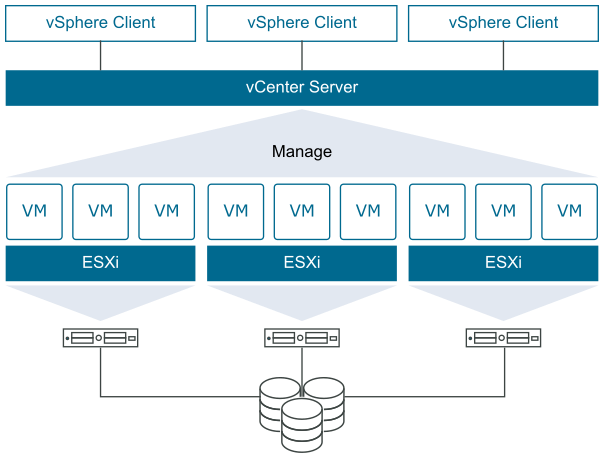
\includegraphics[scale = 0.75]{images/vmware-infrastructure-relationship.png}
    \caption{vSphere's Sotftware Suite Relationship}
    \label{VMware}
\end{figure}

\subsection{ESXi}
\href{https://www.vmware.com/products/esxi-and-esx.html}{ESXi} is a type-1, bare-metal hypervisor that is installed directly on a server and functions as the primary operating system. 

Unlike traditional operating systems (e.g., Linux, Windows Server), ESXi focuses solely on allowing virtualization. While traditional operating systems require the installation of a separate software-based type-2 hypervisor for virtualization, ESXi integrates virtualization directly into the operating system itself.

It's important to note that while ESXi enables virtualization at the OS level, the management of virtualization itself is facilitated through VMware's vSphere suite. vSphere provides the tools and features necessary to create, manage, and optimize virtualized environments. It serves as the management layer for the virtualization capabilities enabled by ESXi.

\begin{figure}[H]
    \centering
    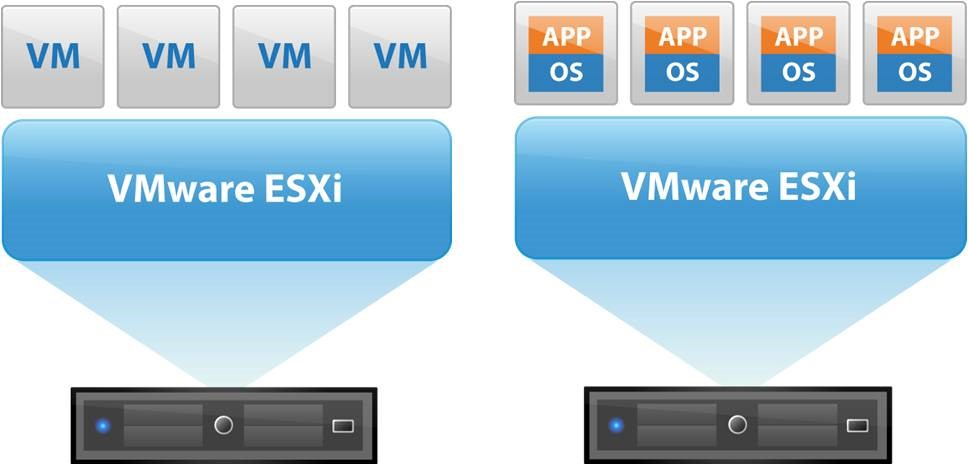
\includegraphics[scale = 0.55]{images/esxi.jpg}
    \caption{ESXi \textcolor{red}{(STOLEN EXAMPLE)} }
    \label{ESXi}
\end{figure}

\subsection{vSphere Client}
The \href{https://docs.vmware.com/en/VMware-vSphere/7.0/com.vmware.vsphere.vcenterhost.doc/GUID-A618EF76-638A-49DA-991D-B93C5AC0E2B1.html}{vSphere Client} is an application (interface) that allows you to manage and monitor your VMware environments. It is important to note that the actual management capabilities stem from the vCenter Server and \textbf{NOT} from vSphere client.

\begin{figure}[H]
    \centering
    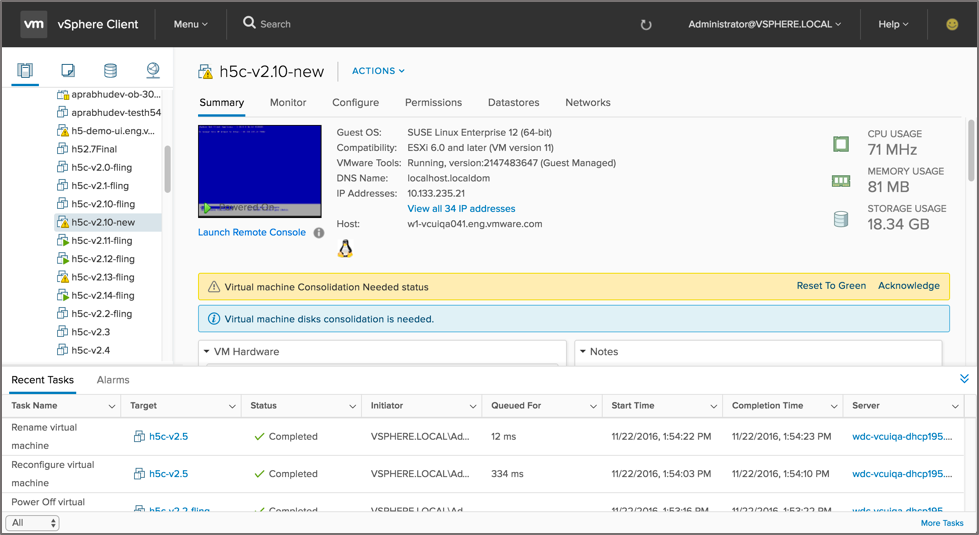
\includegraphics[scale = 0.9]{images/vsphere-client.jpg}
    \caption{vSphere Client \textcolor{red}{(STOLEN EXAMPLE)} }
    \label{vSphere Client}
\end{figure}

\subsection{vCenter}
The vCenter Server is a centralized platform for managing vSphere environments. 

While vSphere serves as the foundation for virtualization, vCenter Server extends these capabilities by acting as a centralized platform designed to manage vSphere environments. Beyond the basic management features offered by vSphere, vCenter Server offers advanced functionalities such as automation, orchestration, and policy-based management.

Some key features of vCenter include: VM migration, security groups, role policies, single sign-on, workflow automation, monitoring and auditing reports, distributed resource management, and optimized resource allocation.

\subsubsection{vCenter Security and Risks}
Security is a critical aspect of virtualized environments, and vCenter provides a range of security features to protect against unauthorized access, data theft, and data manipulation. These security features include: role-based access control\footnote{Define roles and permissions to users based on their roles to prevent unauthorized access.}, auditing\footnote{Track user activity and changes to identify security issues and log actions taken within the virtualized environment.}, encryption\footnote{Encrypt VM data, configuration files, and communication between hosts.}, secure communication\footnote{Supports SSL/TLS encryption to secure communication between hosts and the vCenter server.}, integration\footnote{Integrate with third-party security products (e.g., antivirus, IDS) to provide additional layers of security}, and two-factor authentication\footnote{Provide two forms of identification before accessing the VM to prevent unauthorized access.}. These security features help to ensure confidentiality, integrity, and availability of the virtualized infrastructure, a requirement when working with PHI data. 

\subsection{vSAN}
\href{https://docs.vmware.com/en/VMware-vSphere/7.0/com.vmware.vsphere.vsan-planning.doc/GUID-A80526C8-A941-4F84-9D44-D4B8B3914A95.html}{vSAN} is a software-defined storage solution developed by VMware, which allows organizations to create a distributed storage platform that is integrated with vSphere. This provides a highly scalable and available storage infrastructure, using standard hardware.

By creating a shared data store using the internal disks of ESXi hosts in a vSphere cluster, vSAN allows organizations to pool their storage capacity and performance into a single datastore, scaling it easily by adding more hosts to the cluster. vSAN features data replication, erasure coding, and automatic data rebalancing. Additionally, it offers advanced storage services such as deduplication, compression, and encryption, ensuring optimal storage efficiency and security which streamlines storage management, automates routine tasks, and helps to optimize storage utilization and cost savings.

\begin{figure}[H]
    \centering
    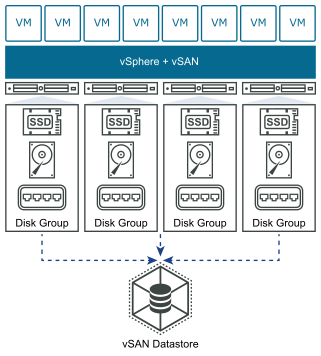
\includegraphics[scale = .8]{images/vsan-deployment.png}
    \caption{Standard vSAN Cluster \textcolor{red}{(STOLEN EXAMPLE)} }
    \label{vSan}
\end{figure}

\subsection{NSX}
\href{https://docs.vmware.com/en/VMware-NSX/index.html}{NSX} is a network virtualization and security platform created by VMware that provides a software-defined networking (SDN) solution that enables organizations to virtualize their network infrastructure, creating a more flexible, scalable, and manageable network.

NSX allows for all network components in your infrastructure to be virtualized, decoupling your network from existing hardware. This abstraction enables organizations to pool and automate network resources, which can reduce the time and cost of deploying and managing network infrastructure. NSX also offers advanced security features and networking capabilities which allows administrators to apply precise policies to specific workloads or applications. For example, NSX provides: network automation, multi-cloud and on-premises support, network segmentation, minimal cost and resource overhead, switching and routing, and load balancing features. 

\begin{figure}[H]
    \centering
    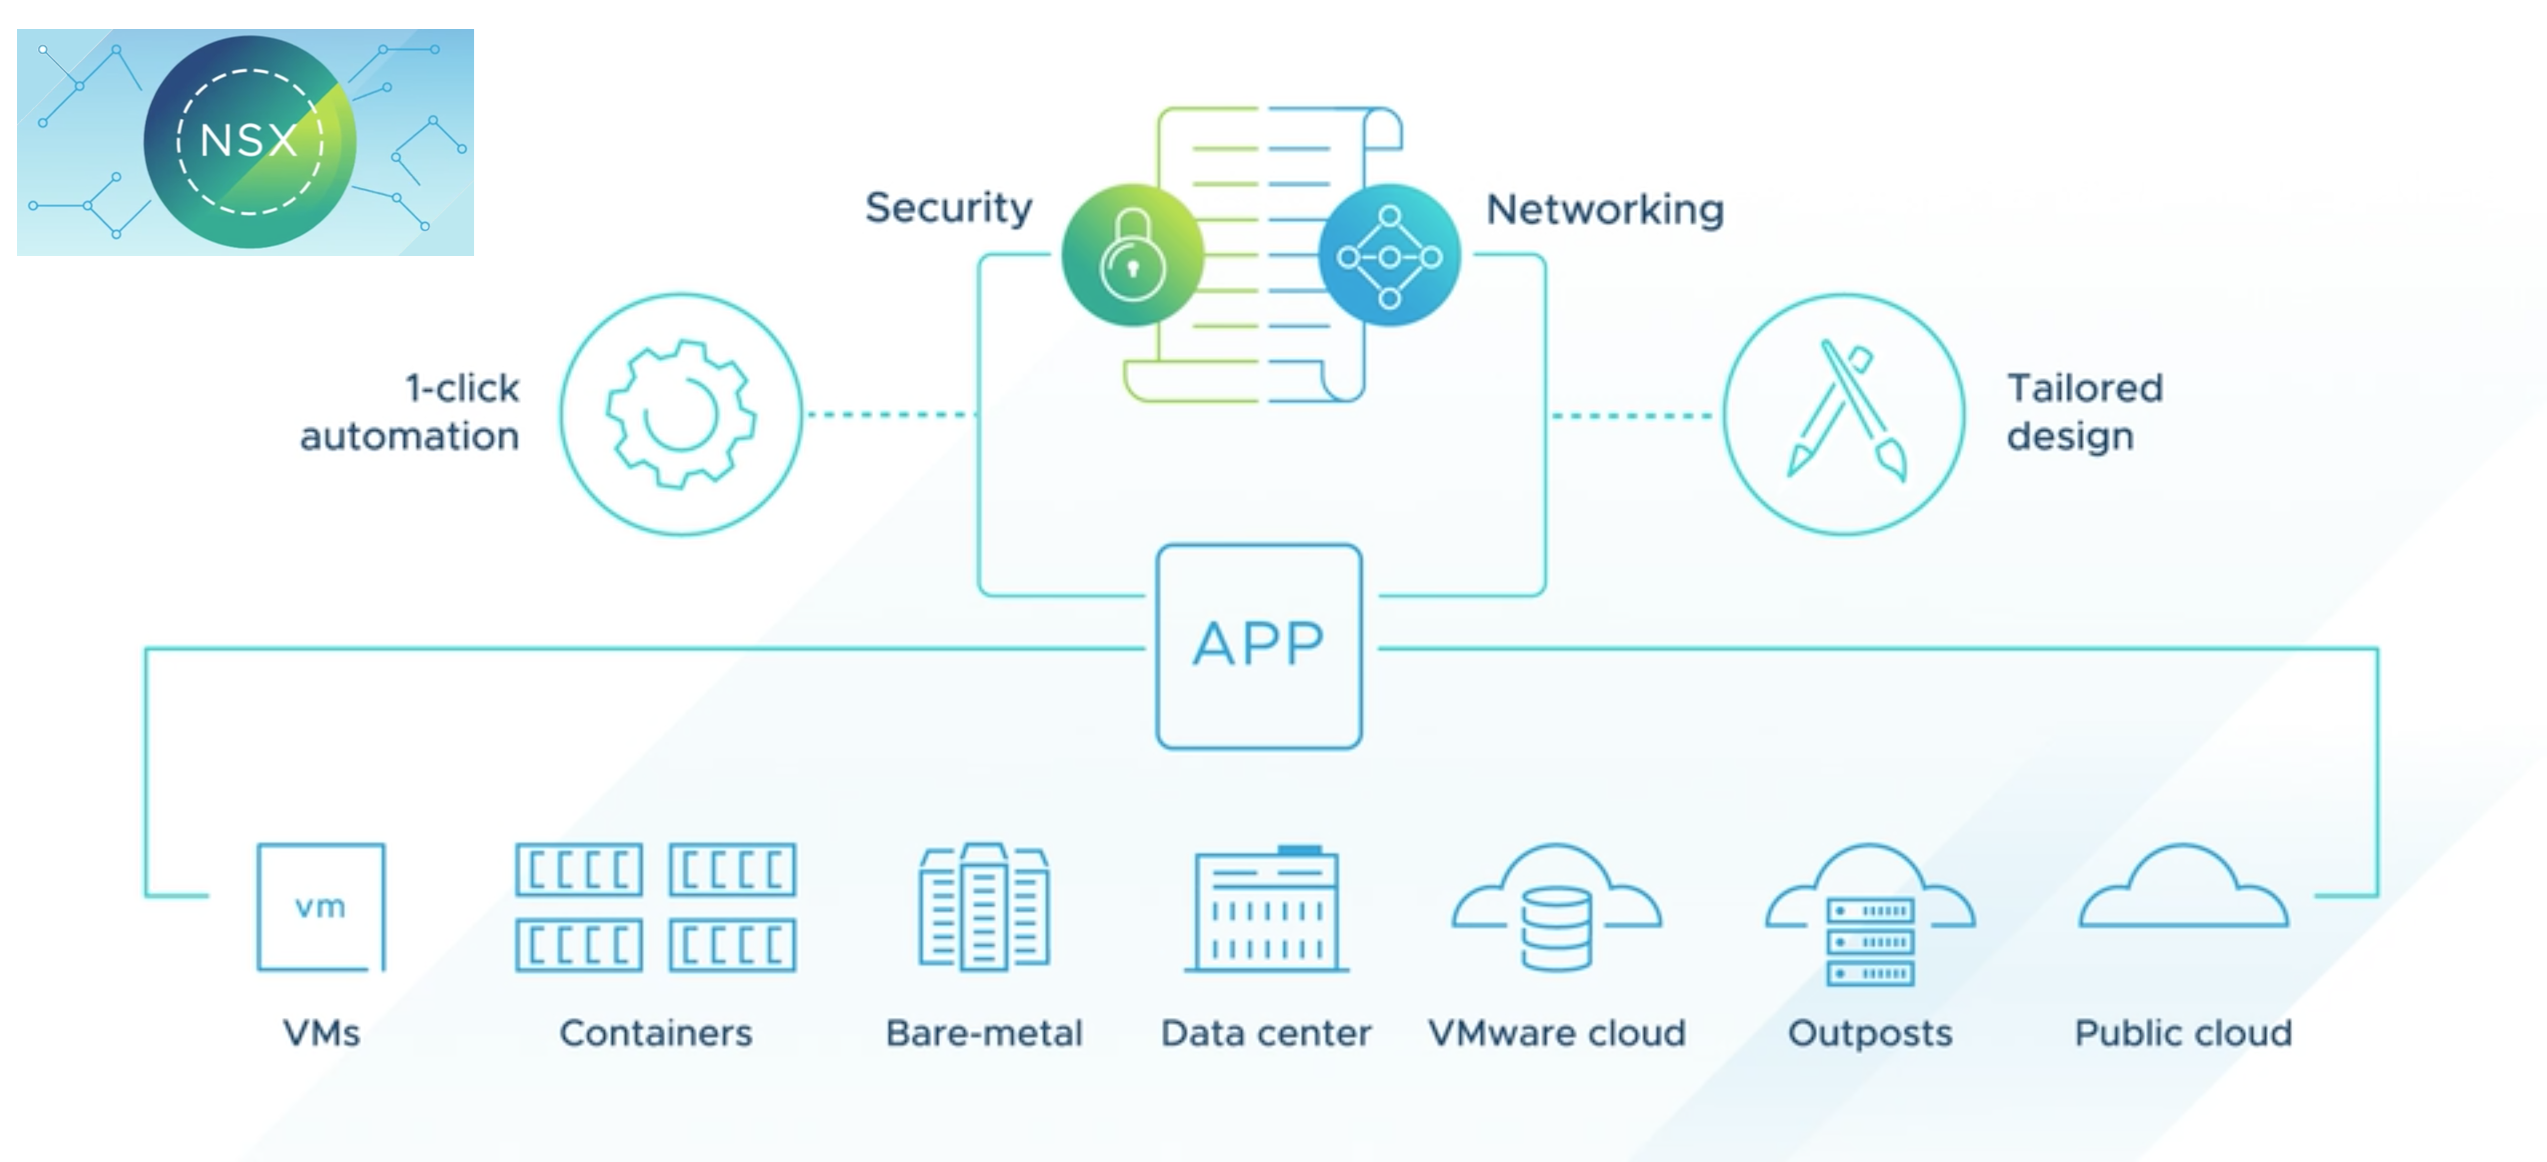
\includegraphics[scale = .19]{images/nsx-diagram.png}
    \caption{NSX Infrastructure \textcolor{red}{(STOLEN EXAMPLE)} }
    \label{NSX}
\end{figure}

\subsection{VMotion}
\href{https://www.vmware.com/products/vsphere/vmotion.html#:~:text=vMotion%20allows%20you%20to%3A,a%20virtual%20machine%20in%20seconds}{VMotion} is virtualization software that enables IT administrators to move VMs between physical servers or hosts without disrupting service. The process involves copying the entire state of the VM, including memory, CPU state, and network connections, from one host to another. The benefits of VMotion include increased availability and uptime, improved hardware utilization, workload balancing, and reduced downtime for maintenance and upgrades. However, the feature also requires specialized hardware and software, increasing the complexity of virtualized environments. VMotion uses shared storage, high-speed networking, and specialized software to ensure a seamless migration. 

The main use case for VMotion is to provide high availability and workload balancing for virtualized environments by optimizing resource usage, improving performance, and avoiding downtime during maintenance or upgrades. For example, an IT administrator can use VMotion to move running VMs to another host during server maintenance, ensuring uninterrupted service for end-users. Once the maintenance is complete, the VMs can be moved back to the original host. VMotion also allows for the consolidation of workloads and the migration of VMs to new hosts for improved hardware utilization and cost savings.

When migrating VMs with sensitive data, such as protected health information (PHI), there may be compliance issues with regulations like HIPAA. To ensure compliance, virtualization infrastructure and VMotion must be configured to meet data protection, access control, and auditability requirements. Encryption and other security measures should also be implemented to protect the confidentiality, integrity, and availability of PHI during migration. IT administrators should ensure that host servers and network connections used for VMotion are secure and protected from unauthorized access.

\begin{figure}[H]
    \centering
    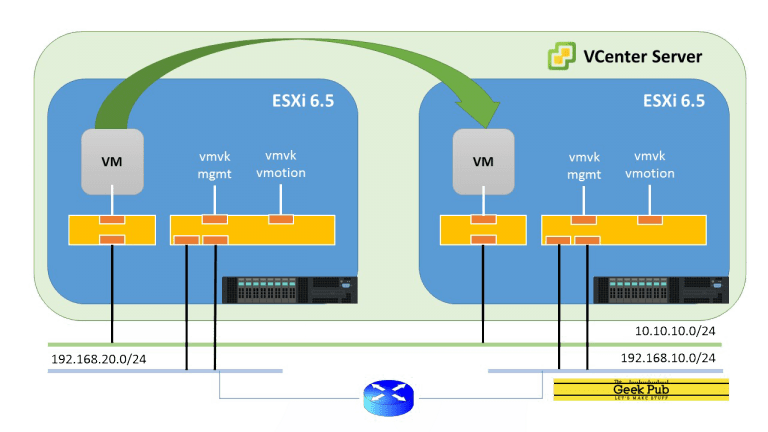
\includegraphics[scale = .50]{images/vmotion.png}
    \caption{VMotion \textcolor{red}{(STOLEN EXAMPLE)} }
    \label{VMotion}
\end{figure}
\newpage

%Creates the SAS section.
\section{Statistical Analysis System (SAS)} \label{section: SAS}
SAS, or Statistical Analysis System, is a software suite that has been used for advanced analytics, business intelligence, data management, and predictive analytics since it was first released in 1976. Developed by the SAS Institute, it offers a range of statistical and data analysis tools, which are suitable for many applications including data mining, forecasting, econometrics, quality control, and statistical analysis.

The software provides a user-friendly graphical interface for data analysis and reporting, as well as a powerful programming language that allows users to customize their analysis and automate repetitive tasks. Its ability to handle large and complex datasets and perform advanced statistical analyses make it popular in various industries, including finance, healthcare, government, and academia. SAS is widely used for purposes such as fraud detection, risk management, clinical research, and marketing analysis, and is a popular choice among data scientists and statisticians. 

SAS offers multiple product\href{https://www.sas.com/en_us/software/all-products.html#all-products-a-z}{\textbf{ suites}}. The SAS Enterprise Suite is a collection of SAS products designed for enterprise-level data management and analysis. The SAS Platform provides two engines for managing foundational capabilities such as distributed processing, security, administration, program development and execution, resource management, user interfaces, cloud integration, operating systems and third-party software. These engines are SAS 9.4 and SAS Visual Analytics. 

In addition to the SAS Enterprise Suite and the SAS Platform, SAS also offers SAS Data Management Advanced which is a powerful ETL solution for preparing data for both analytic engines.

\subsection{SAS Data Management Advanced (SAS DMA)}
SAS Data Management Advanced (SAS DMA), is a software suite that provides a comprehensive set of tools for data integration and data quality. The primary purpose of SAS DMA is to support data ETL (Extract, Transform, Load) processes, which involve extracting data from multiple sources, transforming it to meet specific requirements, and loading it into a target system for analysis and reporting. SAS DMA is a stand-alone software suite and can be deployed on-premises or in the cloud. It is not part of SAS 9.4 (i.e. SAS Data Management and Analytics), which is a separate software suite that provides a wide range of tools for data analysis, reporting, and visualization.

To support these functions, SAS DMA relies on three different types of servers:

\begin{itemize}
    \item The \textbf{Mid-Tier} server is a web-based interface that provides access to SAS DMA workflows. This server is responsible for user authentication and authorization, job scheduling and monitoring, and other functions that are necessary for effective workflow management. It acts as a gateway for users to interact with the SAS DMA system.
    \item The \textbf{Metadata} server is responsible for managing information about data sources and workflows. It provides a central repository for storing metadata, which enables efficient management of SAS objects, definition of relationships between objects, and tracking of changes to data. In the case of SAS DMA, the metadata server manages information about data integration workflows and data quality rules.
    \item The \textbf{Compute} server provides the processing power and resources necessary to run data integration and data quality jobs. This server is responsible for executing the actual data integration and ETL tasks defined in the workflows created in SAS DMA. It ensures that the workflows are run efficiently and effectively, regardless of the size or complexity of the data being processed.
\end{itemize}

\subsection{SAS 9.4}
\href{https://documentation.sas.com/doc/en/pgmsascdc/9.4_3.5/whatsnew/n17cszme3e52b4n1ooe3710fnuec.htm#:~:text=For%20SAS%20administrators%2C%20SAS%209.4,more%20complete%20data%20management%20solution.}{SAS 9.4} is a software suite that provides tools for data management, statistical analysis, business intelligence, and predictive modeling. SAS 9.4 can handle large datasets and complex analyses by using a wide range of built-in functions and procedures that can save time and effort when working with data. 

For example, a pharmaceutical company might use SAS 9.4 to analyze clinical trial data to determine the efficacy and safety of a new drug. A bank might use SAS 9.4 to perform risk analysis on its loan portfolio. A retail company might use SAS 9.4 to analyze customer data to better understand buying patterns and preferences.

SAS 9.4 is composed of several modules that provide a wide range of functionalities:
\begin{itemize}
    \item Base SAS - The basic programming language, data access, and management capabilities of SAS.
    \item SAS/STAT - A comprehensive set of statistical analysis procedures for data exploration and modeling.
    \item SAS/GRAPH - A set of tools for creating high-quality graphical output from SAS data.
    \item SAS/ETS - A set of time series analysis and forecasting procedures.
    \item SAS/IML - An interactive matrix language for matrix manipulation, data analysis, and numerical optimization.
    \item SAS/ACCESS - Connectivity to data sources such as relational databases and spreadsheets.
    \item SAS Enterprise Guide - A graphical user interface (GUI) for SAS programming, data management, and reporting.
\end{itemize}

\subsection{SAS Visual Analytics (SAS Viya)}
SAS Visual Analytics (\href{https://documentation.sas.com/doc/en/pgmsascdc/9.4_3.5/pgmsasgswlcm/home.htm}{SAS Viya}), is a cloud-based analytics platform that provides a suite of tools and services for elastic, scalable, and fault-tolerant data analytics, data processing, and machine learning for enterprise environments. It allows organizations to store, manage, analyze, and share large volumes of data across different sources and formats, all within a single platform. 

SAS Viya is composed of several software that provide a wide range of functionalities:

\begin{itemize}
    \item SAS Visual Analytics: A tool for creating interactive reports and dashboards to explore and visualize data.
    \item SAS Visual Statistics: A tool for performing statistical analysis and building predictive models on large data sets.
    \item SAS Visual Data Mining and Machine Learning: A tool for exploring and analyzing large data sets using advanced analytics techniques such as clustering, decision trees, and neural networks.
    \item SAS Visual Forecasting: A tool for creating accurate and reliable forecasts using time series data.
    \item SAS In-Memory Statistics: A tool for performing high-performance analytics and modeling on large data sets using in-memory processing.
\end{itemize}

When performing analytics on large datasets, SAS Viya uses Cloud Analytic Services.

\subsection{Cloud Analytics Services (CAS)}
Cloud Analytics Services (\href{https://documentation.sas.com/doc/en/calcdc/3.3/calserverscas/n05000viyaservers000000admin.htm}{CAS}) is the in-memory analytics engine SAS Viya uses for both on-premise as well as cloud-service environments (e.g., AWS, Azure, GCP). CAS uses a combination of hardware and software where data management and analytics take place on either a single-machine or as a distributed server across multiple machines. In either single or distributed deployment, each machine (host, node, etc) will be assigned one of three roles: CAS Controller, CAS Backup Controller, CAS Worker.

\textbf{Analogy}
\\
In a restaurant kitchen, there exists three primary chefs. They are the (1) executive chef, (2) sous chef, and (3) station chef(s). The executive chef's primary role is to manage the kitchen and its staff whilst doing very little cooking. The sous chef's primary role is to be the right-hand to the executive chef, ready to manage the kitchen, share, or take over the responsibility of the executive chef at a moments notice. The station chef(s) merely wait for instructions from the executive chef, then executes the job they are given. 

This is the relationship of each CAS node with each other:
\begin{itemize}
    \item The CAS Controller is the executive chef managing the kitchen and its staff, delegating work.
    \item The CAS Backup Controller is the sous chef ready to take over the responsibility of the executive chef. 
    \item The CAS Worker(s) are the station chefs cooking what they are assigned to by the executive chef. 
\end{itemize}

\subsubsection{Role 1: CAS Controller}
Controller is the first role that can be assigned to a host for SAS Cloud Analytic Services. For both server architectures, single-machine and distributed, one machine must be designated as the Controller. The role of the Controller is to parse out work to each Worker host available. In other words, the Controller manages and controls the overall operation of the CAS environment. As the master node, the Controller is responsible for distributing workload among available CAS Workers, managing user sessions, and providing a secure environment for data retrieval and data storage. 

In a single-machine environment, the CAS Controller and CAS Worker roles can be performed by different processes or threads within the same operating system instance. However, we are not limited to this deployment method as it is also possible to have the CAS Controller and CAS Worker(s) virtually separated (on the same hardware) to increase the scalability of the deployment. The configuration of your architecture depends on what you need out of CAS.  

In a distributed environment, the CAS Controller is responsible for managing and controlling the CAS environment whilst the actual data processing and data analytics are performed by the CAS Worker(s).
%insert diagram%

\subsubsection{Role 2: CAS Backup Controller}
Backup Controller is the second role that can be assigned to a host for SAS Cloud Analytic Services. Although optional, the CAS Backup Controller is highly recommended in a distributed server environment. The role of the CAS Backup Controller is to act as a standby or hot-backup for the primary CAS Controller in case of a failure. Its primary purpose is to ensure that the system can continue to function in the event of a failure of the primary controller. The Backup Controller is typically set to passively monitor the primary controller for any signs of failure, such as a loss of connectivity or failure to respond to heartbeat messages. It does not actively participate in task scheduling or job execution while the primary controller is running normally. 

If the primary CAS Controller fails, the Backup Controller will take over as the primary controller and assume responsibility for managing the CAS worker nodes and scheduling tasks. In this scenario, the CAS worker nodes will send their status updates and job results to the Backup Controller instead of the failed primary controller.\footnote{If the main CAS Controller fails, how does each CAS Worker respond to the Backup Controller with their completed jobs?}

In some systems, the Backup Controller can also be given jobs to execute as a CAS worker node. This can help to improve the system's overall performance by increasing the number of available processing resources. In this scenario, the Backup Controller can perform both the role of a CAS Controller and a CAS worker node.\footnote{Can the CAS Backup Controller be assigned work as well as passively monitor the main CAS Controller?}

%insert diagram%

\subsubsection{Role 3: CAS Workers}
Worker is the third role that can be assigned to a host for SAS Cloud Analytic Services. The CAS Worker is responsible for performing data processes and data analytics sent from the CAS Controller. For example, CAS Workers can perform data manipulations, transformations or computations on large/complex datasets. These computations are but not limited to: statistical analysis, machine learning models, text analysis, time series analysis, optimization, etc. Workers execute these computations using data stored on disk, in-memory, or in a distributed file system. 

In a distributed environment, one host will be assigned as your controller and any additional hosts are considered workers (optional CAS Backup Controller). Workers increase the overall computing power of your distributed-server and provides a solution for a scalable (up/down), distributed, and fault-tolerant environment for data storage and data analysis because the worker manages the storage of data/metadata across multiple nodes. The amount of CAS Workers needed to create an optimized distributed environment is highly dependant on data size, computation type, and workload.  
%insert diagram%

We can create two types of CAS configurations: a single-machine environment using symmetric multiprocessing \href{https://documentation.sas.com/doc/en/calcdc/3.3/calserverscas/n05000viyaservers000000admin.htm}{\textbf{(SMP)}}, or distributed server environment using massively parallel processing \href{https://documentation.sas.com/doc/en/calcdc/3.3/calserverscas/n05000viyaservers000000admin.htm}{\textbf{{(MPP)}}}.

\subsubsection{Symmetric Multiprocessing (SMP)}
The Symmetric multiprocessing (SMP) architecture is used when you want to run CAS on a single server or virtual machine (VM) with multiple CPU cores. This is called shared-memory architecture because all the CPUs share the same memory. When a job is submitted to CAS in an SMP architecture, it is processed by the worker node(s) in parallel using the shared memory. The results are returned to the controller node, which sends them back to the user.

A typical SMP architecture for CAS might consist of a single VM that serves as both the controller and worker node. The number of VMs required will depend on the size of your data and the processing requirements of your workload. For example, if you have a large dataset or complex analytical workloads, you might deploy CAS on a VM with 8 or 16 CPU cores.

Some examples of use cases for CAS on an SMP architecture include:

\begin{itemize}
    \item Exploratory data analysis
    \item Statistical modeling and regression analysis
    \item Predictive analytics
    \item Machine learning and deep learning
\end{itemize}

\begin{figure}[H]
    \centering
    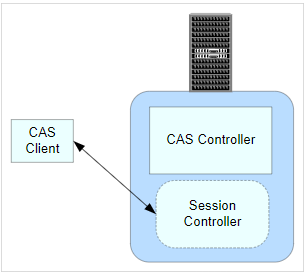
\includegraphics[scale = 0.8]{images/smp_server.png}
    \caption{Single-machine CAS Server \textcolor{red}{(STOLEN EXAMPLE)} }
    \label{SMP Achitecture}
\end{figure}

\subsubsection{Massively Parallel Processing (MPP)}
The Massively Parallel Processing (MPP) architecture is used when you want to run CAS on a cluster of multiple servers or VMs. This is called distributed-memory architecture because the data is partitioned and stored across multiple servers or nodes. When a job is submitted to CAS in an MPP architecture, it is distributed across the worker nodes in parallel. Each worker node processes its own subset of the data and returns the results to the controller node. The controller node then aggregates the results from all worker nodes and sends them back to the user.

A typical MPP architecture for CAS might consist of multiple VMs or servers, with some dedicated as controller nodes and others as worker nodes. The number of VMs or servers required will depend on the size of your data and the processing requirements of your workload. For example, you might choose to deploy CAS on a cluster of 10 or more VMs or servers to handle large-scale data processing tasks.

Some examples of use cases for CAS on an MPP architecture include:
\begin{itemize}
    \item Big data processing and analysis
    \item High-performance computing
    \item Large-scale machine learning and deep learning
    \item High-throughput data processing, such as in genomics or drug discovery
\end{itemize}

\begin{figure}[H]
    \centering
    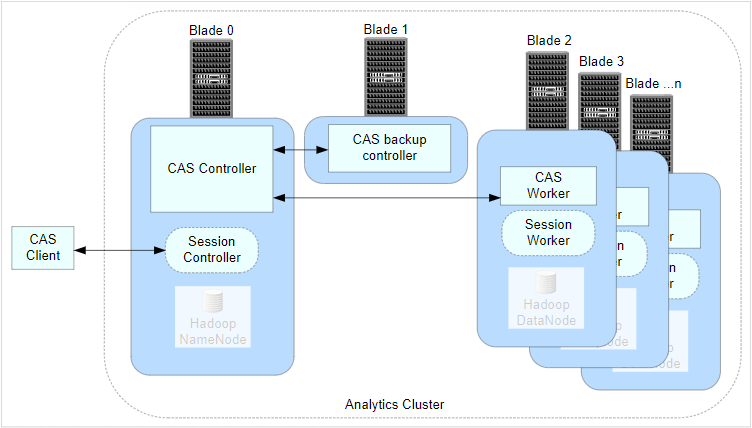
\includegraphics[scale = 0.70]{images/mpp_server.png}
    \caption{Distributed CAS Server \textcolor{red}{(STOLEN EXAMPLE)} }
    \label{MMP Architecture}
\end{figure}


\newpage

%Creates the Massively Learning Activities section.
\section{Security and Risk Management} \label{section: SARM}
This chapter provides an introduction to security and risk management by covering key concepts such as data compliance, identity and access management (IAM), data governance, data encryption, and data backups. This chapter is not intended to be a comprehensive handbook for implementing proper security measures, but rather as an overview of the security measures to consider when developing a strategy for storing and accessing sensitive information.

\subsection{Data Compliance}

\begin{itemize}
    \item HIPAA Compliance
    \item UHM Compliance
    \item RCUH Compliance
    \item TASI Compliance
    \item State of Hawaii Compliance
\end{itemize}

\subsection{Identity and Access Management (IAM)}
Identity and Access Management (IAM) is a security practice that safeguards sensitive information by allowing only authorized individuals to access confidential resources and data. 

Identity management looks to confirm that an accessing user is who they say they are, whilst access management uses a users identity to determine which resource they are allowed to access. 

IAM components can be classified into four major categories: authentication, authorisation, user management, and central user repository.

\subsubsection{Authentication}
Authentication is a component of IAM in which a user is required to provide sufficient credentials to gain access to an application system. 

Sufficient credentials for accessing sensitive healthcare information are defined as authentication methods that comply with the HIPAA Security Rule (Section 5.1). The HIPAA Security Rule requires covered entities to implement multi-factor authentication or an equivalent authentication method for accessing ePHI.

According to HIPAA, the multi-factor authentication method must use two of the following three elements:

\begin{itemize}
    \item Something you know (Password or PIN)
    \item Something you have (Smart Card or Security Token) 
    \item Something you are  (Fingerprint or Facial Recognition)
\end{itemize}

Two new additional standards are not required but provide additional authentication methods:

\begin{itemize}
    \item Somewhere you are (IP Address or Geo-location)
    \item Something you do (Signature or Gesture)
\end{itemize}

Once a user is authenticated, a session is created to allow the user to interact with the application system. The session will remain open until the user's task is completed or through termination by other means (e.g., timeout). By centrally maintaining the session of a user, the authentication module can provide single sign-on services. 

Single sign-on (SSO) is a mechanism that allows users to authenticate once and access multiple systems or applications without having to re-enter their credentials. SSO simplifies access control and user permissions by providing a centrally managed solution for user authentication policies across all systems. There are several options when deciding on a SSO solution. (e.g., LDAP, OAuth, SAML, RADIUS, PKI, etc).

\subsubsection{Authorization}
Authorization is a component of IAM in which a user is given permission to access a particular resource. 

This component comes after a user has successfully authenticated to an application system with sufficient credentials. Authorization is performed by checking the resource access request (e.g., web-based application URL), against an IAM policy store and is the core module that implements Role-Based/Attribute-based, access control. 

\begin{itemize}
    \item Role-Based Access Control (RBAC) is a method of access control that assigns roles to users  and access permissions to those roles in order to provide a centrally managed solution for authorization. 
    \item Attribute-Based Access Control (ABAC) is a method of access control that assigns permissions based on a user's attributes (e.g., job title, location, department). 
\end{itemize}

The authorization model can provide more complex access control policies other than user role/groups and user attributes (e.g., access channels, time, resource requested, external data, business rules). 

\subsubsection{Central User Repository}
The Central User Repository (CUR) stores and delivers identity information in order to verify credentials submitted from clients. Identity information is equivalent to user account information (e.g., usernames, passwords, etc). The most common CUR protocol is the Lightweight Directory Access Protocol (LDAP). 

LDAP is a protocol for accessing and maintaining distributed directory information services over an Internet Protocol network in order to provide a centrally managed authentication and authorization solution for application systems. 

LDAP allows system administrators to manage user accounts, configure access and permissions, and monitor and audit user activity.

\begin{figure}[H]
    \centering
    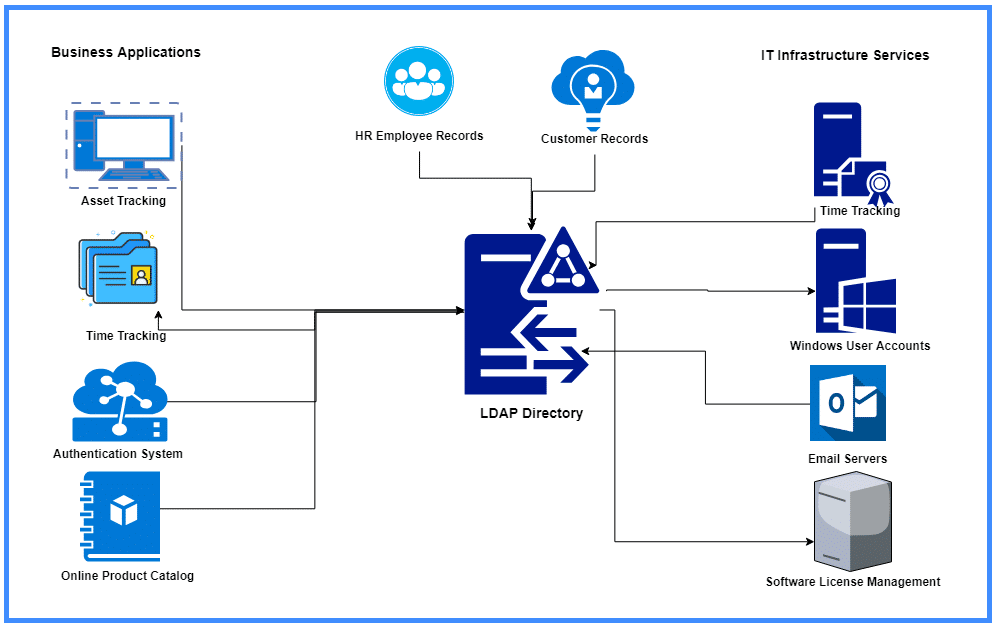
\includegraphics[scale = 0.6]{images/LDAP.png}
    \caption{Lightweight Directory Access Protocol \textcolor{red}{(STOLEN EXAMPLE)} }
    \label{LDAP}
\end{figure}

When designing an LDAP directory, it is important to consider the principle of least privilege. The principle of least privilege is a design principle where each user or service is only given the necessary permissions to perform their intended tasks, and no more. Unauthorized users should not access important data or systems. The principle of least privilege should also be considered when designing security groups and access control lists, as unauthorized users must not have access to sensitive information.

\subsubsection{User Management}

User Management is the component of IAM that covers the creation and maintenance of user accounts, account identity, and account privileges. 

Identity creation and maintenance is controlled by the set of administrative functions such as user life-cycle management, role/group management, and user/group provisioning. User life-cycle management controls the lifespan of user accounts from account provision to account deprovision. Role/group management and user/group management is used for user authorization (Section 5.2.2). 

Onboarding, maintenance, and off-boarding are the three components of user life-cycle management. 

\begin{enumerate}
    \item On-boarding Process:
        \begin{itemize}
            \item Account authentication for relevant systems and applications.
            \item Verification of tenant identity.
            \item Setting up multi-factor authentication.
            \item Domain and network access configuration.
            \item Training for new tenants on how to use the systems and applications they have access to.
        \end{itemize}
    \item Maintenance Process:
        \begin{itemize}
            \item Regular review of tenant access privileges to ensure that they align with the tenant's job function and level of responsibility.
            \item Management of access requests and approvals to ensure that access is only granted to authorized tenants.
            \item Management of tenant accounts and passwords, including password expiration policies and periodic password resets.
            \item Monitoring and auditing tenant activity to detect for potential security threats.
            \item Provisioning of additional access or permissions based on changes to the tenant's role or job function.
        \end{itemize}
    \item Off-boarding Process:
        \begin{itemize}
            \item Revocation of tenant access to all systems and applications once life-cycle is expired. 
            \item Archiving or removal of tenant data in accordance with the organizations (e.g., TASI, RCUH, UHM, etc.) policies and regulatory requirements.
            \item Review of tenant access to ensure that no data or resources have been left behind.
            \item Disabling or revocation of any credentials associated with the tenant's access.
            \item Notification of relevant stakeholders about the tenant's departure.
        \end{itemize}
\end{enumerate}

\subsection{Data Governance}
\textcolor{red}{\textbf{To be completed during the Data Governance Seminar in early May 22-24, 2023.}}

\subsection{Data Encryption}

Data Encryption is a security practice that safeguards sensitive information by transforming the data into an unreadable format that can only be deciphered with the appropriate decryption key. 

HIPAA Security Rule (Section 5.1) requires covered entities to implement a mechanism to encrypt and decrypt ePHI based on the assessment of risks to the confidentiality, integrity, and availability of the ePHI. 

\begin{itemize}
    \item Data At-Rest is data that is stored in storage devices (e.g., disk, tap, USB drives, non-votalite storage, etc) and is not being used or transmitted.
    \item Data In-Transit is data that is transmitted over a network (e.g., file transfers, emails, instant messages). HIPAA requires the use of secure transmission protocols (e.g., SSL, TLS) for transmitting ePHI over public networks. 
\end{itemize}

\subsection{Data Backup}

A Data Backup is a copy of data that is used for data restoration in the case of data loss, data corruption, or other data-related disasters.

\begin{itemize}
    \item Recovery Point Objective (RPO) is the maximum amount of data – as measured by time – that can be lost before data loss exceeds what is acceptable to an organization.
    \item Recovery Time Objective (RTO) is the maximum tolerable length of time that a system (e.g., can be down after a failure or disaster occurs. 
\end{itemize}


\newpage

%Creates the Massively Learning Activities section.
\section{Massively Learning Activities I - Initial Deployment} \label{section: MLA}
The System Development Life-cycle (SDLC) is a project management model that defines different stages that are necessary to bring a project from conception to deployment and later maintenance. The SDLC model consists of several phases: planning, requirement gathering, design, implementation, testing \& integration, and operations \& maintenance. It provides a systematic approach to system development that helps ensure that system is built efficiently with minimal risk.

Massively Learning Activities will follow a similar variation to the SDLC project management model where each SDLC stage will correspond to a subsection in this chapter.

\begin{figure}[H]
    \centering
    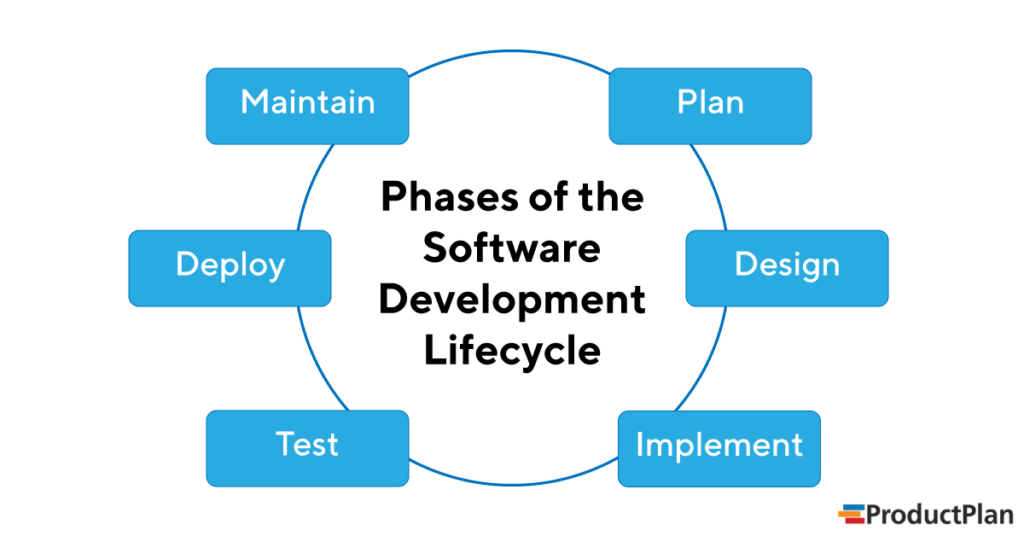
\includegraphics[scale = 0.25]{images/SDLC_Framework.png}
    \caption{System Developerment Life-Cycle \textcolor{red}{(STOLEN EXAMPLE)} }
    \label{SDLC}
\end{figure} 

%----------------------------------------------------------------------------------%

\subsection{Planning I} 

TASI has been contracted by CNMI to create an infrastructure that will allow for data analytics on Protected Health Information (PHI). To achieve this, TASI will provide a Platform as a Service (PaaS) solution, by hosting SAS services on on-premises hardware, configured for multi-tenancy.

Tenants will provide the data, which will be submitted through an ETL pipeline for data migration, cleaning, and processing. Once the data has been processed, tenants may perform data analytics using advanced algorithms in SAS programming language.

Due to SAS being a time sensitive project, the initial deployment will have SAS suites and VMs installed on existing hardware, with plans to migrate the infrastructure to newly acquired hardware in the future.

MLA I will expect 4 tenants:
\begin{enumerate}
    \item Commonwealth of the Northern Mariana Islands (CNMI)
    \item All-Payer Claims Database (APCD)
    \item Centers for Medicare \& Medicaid Services (CMA)
    \item Med-Quest
\end{enumerate}

\subsection{Requirement of Analysis I}

The Requirement Analysis phase is a crucial component in developing a robust SAS infrastructure using the SDLC framework. This phase involves gathering and analyzing the specific requirements for the project, including pre-installation checklists and EEC sizing requirements. In this phase, ongoing project management tasks will be performed, such as preparing a project plan and assigning appropriate resources. 

Furthermore, as part of this phase, SAS will send a Pre-Install Requirements Document to the client for completion, and both parties will ensure environmental readiness for installation by reviewing the completed document. 

Additionally, SAS will send a billable work hours log for verification based on the project plan. This subsection will provide a detailed overview of the pre-installation checklist and EEC sizing requirements necessary for a successful implementation of the SAS infrastructure.

\newpage 

\subsubsection{Multi-Tenancy Configuration Plan: VM Location}
\label{Multi-Tenancy Configuration Plan}

\begin{figure}[H]
\begin{center}
    \renewcommand{\arraystretch}{1.5}
    \begin{tabular}{|>{\raggedright\arraybackslash}l 
                    |>{\raggedright\arraybackslash}m{6cm} 
                    |>{\raggedright\arraybackslash}l 
                    |>{\raggedright\arraybackslash}l 
                    |>{\raggedright\arraybackslash}l 
                    |}
    \hline
    \rowcolor[HTML]{196fb4}\centering\textcolor{white}{\large Server Name} 
                            & \centering\textcolor{white}{\large Function} 
                            & \centering\textcolor{white}{\large Type} 
                            & \centering\textcolor{white}{\large Site} 
                            & \centering\textcolor{white}{\large Physical Server} 
                            \tabularnewline 
    \hline
    DC1	           & LDAP Host1                         & VM & ITS M01 & FX2Blade4 \\\hline
    DC2	           & LDAP Host2                         & VM & ITS M01 & FX2Blade1 \\\hline
    SAS 9.4 Server & SAS Infrastructure Server          & VM & ITS M01 & FX2Blade2 \\\hline
    SAS DMA	       & SAS Data Management Advanced       & VM & ITS M01 & NaN	\\\hline
    SAS Ansible	   & Ansible	                        & VM & ITS M01 & NaN	\\\hline
    SAS PRT	       & SAS Programming Run-Time	        & VM & ITS M01 & NaN	\\\hline
    SAS SL	       & SAS Service Layer	                & VM & ITS M01 & NaN	\\\hline
    Provider CC1   & Provider Primary CAS Controller    & VM & ITS M01 & NaN	\\\hline
    Provider CC1   & Provider Backup CAS Controller     & VM & ITS M01 & NaN	\\\hline
    R1 CC1	       & Research 1 CAS Controller 1	    & VM & ITS M01 & NaN	\\\hline
    R1 CC2	       & Research 1 CAS Controller 2	    & VM & ITS M01 & NaN	\\\hline
    R1 W1	       & Research 1 CAS Worker 1	        & VM & ITS M01 & NaN	\\\hline
    R1 W2	       & Research 1 CAS Worker 2	        & VM & ITS M01 & NaN	\\\hline
    R1 W3	       & Research 1 CAS Worker 3	        & VM & ITS M01 & NaN	\\\hline
    R2 CC1	       & Research 2 CAS Controller 1	    & VM & ITS M01 & NaN	\\\hline
    R2 CC2	       & Research 2 CAS Controller 2	    & VM & ITS M01 & NaN	\\\hline
    R3 W1	       & Research 3 CAS Worker 1	        & VM & ITS M01 & NaN	\\\hline
    R3 W2	       & Research 3 CAS Worker 2	        & VM & ITS M01 & NaN	\\\hline
    R3 W3	       & Research 3 CAS Worker 3	        & VM & ITS M01 & NaN	\\\hline
    R4 CC1	       & Research 4 Primary CAS Controller  & VM & ITS M01 & NaN	\\\hline
    R4 CC2	       & Research 4 Backup CAS Controller   & VM & ITS M01 & NaN	\\\hline
    R4 W1	       & Research 4 CAS Worker 1	        & VM & ITS M01 & NaN	\\\hline
    E1 CC1	       & Education 1 Primary CAS Controller & VM & ITS M01 & NaN	\\\hline
    E1 CC2	       & Education 1 Backup CAS Controller  & VM & ITS M01 & NaN	\\\hline
    E1 W1	       & Education 1 CAS Worker 1	        & VM & ITS M01 & NaN	\\\hline
    E2 CC1	       & Education 2 Primary CAS Controller & VM & ITS M01 & NaN	\\\hline
    E2 CC2	       & Education 2 Backup CAS Controller  & VM & ITS M01 & NaN	\\\hline
    E2 W1	       & Education 2 CAS Worker 1	        & VM & ITS M01 & NaN	\\\hline
    E3 CC1	       & Education 3 Primary CAS Controller & VM & ITS M01 & NaN	\\\hline
    E3 CC2	       & Education 3 Backup CAS Controller  & VM & ITS M01 & NaN	\\\hline
    E3 W1	       & Education 3 CAS Worker 1	        & VM & ITS M01 & NaN	\\\hline
    E4 CC1	       & Education 4 Primary CAS Controller & VM & ITS M01 & NaN	\\\hline
    E4 CC2	       & Education 4 Backup CAS Controller  & VM & ITS M01 & NaN	\\\hline
    E4 W1	       & Education 4 CAS Worker 1	        & VM & ITS M01 & NaN	\\\hline
    
    \end{tabular}
\end{center}
\caption{Physical and logical locations of VMs related to SAS technologies.}
\label{MTP-1}
\end{figure}

\subsubsection{Multi-Tenancy Configuration Plan: Resource Allocation}

\begin{figure}[H]
\begin{center}
    \renewcommand{\arraystretch}{1.5}
    \begin{tabular}{|>{\raggedright\arraybackslash}l 
                    |>{\raggedright\arraybackslash}l
                    |>{\raggedright\arraybackslash}l 
                    |>{\raggedright\arraybackslash}m{2cm}
                    |>{\raggedright\arraybackslash}l 
                    |>{\raggedright\arraybackslash}m{2cm} 
                    |>{\raggedright\arraybackslash}m{1.5cm} 
                    |}
    \hline
    \rowcolor[HTML]{196fb4}\centering\textcolor{white}{\large Server Name} 
                            & \centering\textcolor{white}{\large Tenant} 
                            & \centering\textcolor{white}{\large OS} 
                            & \centering\textcolor{white}{\large Memory (GB)} 
                            & \centering\textcolor{white}{\large vCPU}
                            & \centering\textcolor{white}{\large Min Sys Storage}
                            & \centering\textcolor{white}{\large Storage (GB)}
                            \tabularnewline 
    \hline
    DC1	           & NaN      & RHEL 8 & 12 & 4 & NaN & 50  \\\hline
    DC2	           & NaN      & RHEL 8 & 12 & 4 & NaN & 50  \\\hline
    SAS 9.4 Server & NaN      & RHEL 8 & 32 & 8 & NaN & NaN \\\hline
    SAS DMA	       & NaN      & RHEL 8 & 32 & 8 & NaN & NaN \\\hline
    SAS Ansible	   & NaN	  & RHEL 8 & 16 & 2 & NaN & NaN \\\hline
    SAS PRT	       & NaN	  & RHEL 8 & 64 & 6 & NaN & NaN \\\hline
    SAS SL	       & NaN	  & RHEL 8 & 32 & 2 & NaN & NaN \\\hline
    Provider CC1   & Provider & RHEL 8 &  8 & 2 & NaN & NaN \\\hline
    Provider CC1   & Provider & RHEL 8 &  8 & 2 & NaN & NaN \\\hline
    R1 CC1	       & Tenant 1 & RHEL 8 & 16 & 2 & NaN & NaN \\\hline
    R1 CC2	       & Tenant 1 & RHEL 8 & 16 & 2 & NaN & NaN \\\hline
    R1 W1	       & Tenant 1 & RHEL 8 & 16 & 2 & NaN & NaN \\\hline
    R1 W2	       & Tenant 1 & RHEL 8 & 16 & 2 & NaN & NaN \\\hline
    R1 W3	       & Tenant 1 & RHEL 8 & 16 & 2 & NaN & NaN \\\hline
    R2 CC1	       & Tenant 2 & RHEL 8 & 16 & 2 & NaN & NaN \\\hline
    R2 CC2	       & Tenant 2 & RHEL 8 & 16 & 2 & NaN & NaN \\\hline
    R3 W1	       & Tenant 2 & RHEL 8 & 16 & 2 & NaN & NaN \\\hline
    R3 W2	       & Tenant 2 & RHEL 8 & 16 & 2 & NaN & NaN \\\hline
    R3 W3	       & Tenant 2 & RHEL 8 & 16 & 2 & NaN & NaN \\\hline
    R4 CC1	       & Tenant 3 & RHEL 8 &  8 & 1 & NaN & NaN \\\hline
    R4 CC2	       & Tenant 3 & RHEL 8 &  8 & 1 & NaN & NaN \\\hline
    R4 W1	       & Tenant 3 & RHEL 8 &  8 & 1 & NaN & NaN \\\hline
    E1 CC1	       & Tenant 4 & RHEL 8 &  8 & 1 & NaN & NaN \\\hline
    E1 CC2	       & Tenant 4 & RHEL 8 &  8 & 1 & NaN & NaN \\\hline
    E1 W1	       & Tenant 4 & RHEL 8 &  8 & 1 & NaN & NaN \\\hline
    E2 CC1	       & Tenant 5 & RHEL 8 &  8 & 1 & NaN & NaN \\\hline
    E2 CC2	       & Tenant 5 & RHEL 8 &  8 & 1 & NaN & NaN \\\hline
    E2 W1	       & Tenant 5 & RHEL 8 &  8 & 1 & NaN & NaN \\\hline
    E3 CC1	       & Tenant 6 & RHEL 8 &  8 & 1 & NaN & NaN \\\hline
    E3 CC2	       & Tenant 6 & RHEL 8 &  8 & 1 & NaN & NaN \\\hline
    E3 W1	       & Tenant 6 & RHEL 8 &  8 & 1 & NaN & NaN \\\hline
    E4 CC1	       & Tenant 7 & RHEL 8 &  8 & 1 & NaN & NaN \\\hline
    E4 CC2	       & Tenant 7 & RHEL 8 &  8 & 1 & NaN & NaN \\\hline
    E4 W1	       & Tenant 7 & RHEL 8 &  8 & 1 & NaN & NaN \\\hline
    \end{tabular}
\end{center}
\caption{Resource requirements of VMs related to SAS technologies.}
\label{MTP-2}
\end{figure}

\subsubsection{EEC Sizing and Pre-Installation Checklist: File Path(s)}

The full EEC Sizing and Pre-Installation Checklist(s) documents can be found in:
\begin{itemize}
    \item PATH: $\backslash$ $\backslash$ .. 300 SAS Installation $\backslash$ 9.4 $\backslash$ EEC Sizing Results
    \item PATH: $\backslash$ $\backslash$ .. 300 SAS Installation $\backslash$ SAS Viya 3.5 $\backslash$ EEC Sizing Results
\end{itemize}

\subsubsection{EEC Sizing: SAS 9.4 (Summarized)}
This document provides sizing guidance for SAS Office Analytics/Data Management Advanced. The estimate provided assumes a typical implementation of SAS Office Analytics/Data Management Advanced and does not take into account any additional workloads or components that may be added. The estimate is based on a preferred hardware vendor with a given performance characteristic. It is recommended that the environment be closely monitored and scaled to support the required workloads to meet the business objectives.

\begin{enumerate}
    
    \item Hardware and Operation System Assumptions:
    \begin{figure}[H]
    \begin{center}
        \renewcommand{\arraystretch}{1.5}
        \begin{tabular}{|>{\raggedright\arraybackslash}m{8cm} 
                        |>{\raggedright\arraybackslash}l
                        |}
        \hline
        \rowcolor[HTML]{196fb4}\centering\textcolor{white}{\large Tier} 
                                & \centering\textcolor{white}{\large Cores$\backslash$RAM} 
                                \tabularnewline 
        \hline
        SAS Metadata Server & \vtop{\hbox{\strut 2 cores with 16GB RAM}
                                    \hbox{\strut (8 GB RAM per core minimum)}}\\\hline
        SAS Compute Server  & \vtop{\hbox{\strut 6 to 8 cores with 48 to 64GB RAM}
                                    \hbox{\strut (8 GB RAM per core minimum)}}\\\hline
        SAS Mid-Tier Server (Web-App Server) 
                            & \vtop{\hbox{\strut 2 cores with 24GB RAM}
                                    \hbox{\strut (24 GB RAM per server minimum)}}\\\hline
        \end{tabular}
    \end{center}
    \caption{Hardware estimate for SAS 9.4: SAS Data Management Advanced. }
    \label{DMA-HRDWR-EST}
    \end{figure}
    \begin{itemize}
        \item This response is based on Intel Xeon E5-2600v4 or Gold 6200/6300 series processor with a clock speed of at least 3.30 GHz running Windows Server 2019, 64 bit operating system.
        \item Core counts are guidelines only. These requirements may vary depending on the solutions installed or the number of users/sessions supported in accordance with Operating System Guidelines and SAS recommendations, page file space should be set to 1.5 to 2 times the amount of physical memory. The machines should be configured for maximum memory bandwidth; this will be dependent on the actual processors/machines selected.
    \end{itemize}
    \item SAS Environment and Configuration Assumptions:
    \begin{itemize}
        \item SAS tends to be I/O intensive. Consider the peak I/O throughput requirements of their system and work with their storage provider to ensure that the storage environment can provide the level of I/O required. A significant percentage of “performance problems” reported to SAS Technical Support can be directly attributed to insufficient levels of I/O throughput.
        \item Recommended I/O throughput rates for the SAS Data and SAS WORK file systems are as follows: for permanent SAS data files, your application throughput requirements may dictate a minimum I/O throughput rate of 100-150 MBs/sec per core, minimum, in the system. Reads and writes to the file system will occur during the ETL process. Chronic and heavy reads and writes are common for the SAS WORK file system. 
        \item Depending on the architecture and deployment, multiple compute tiers need access to a common data area. This may require the use of a centralized storage mechanism such as a Clustered File System (CFS).
    \end{itemize}
\end{enumerate}

This sizing estimate is based on a combination of guidelines provided by SAS R\&D, SAS Product Management, test data, and field experience. Our best practice is to provide the topology as developed by R\&D and try to provide as unified a presentation of the requirements as possible. When questions on deployment arises, the Sizing team defers to the account team.

\subsubsection{EEC Sizing: SAS Viya 3.5 (Summarized)}

This document provides sizing guidance for SAS Viya 3.5. The estimate is not a performance benchmark and does not provide any performance guarantee. The University of Hawai’i at Manoa is responsible for all costs associated with procuring any hardware. This estimate assumes that appropriate data management activities will happen outside of SAS In Memory, and resources for data management activities are not included in this exercise.

\begin{enumerate}
    
    \item Hardware and Resource Assumptions:
    \begin{figure}[H]
    \begin{center}
        \renewcommand{\arraystretch}{1.5}
        \begin{tabular}{|>{\raggedright\arraybackslash}l 
                        |>{\raggedright\arraybackslash}l
                        |}
        \hline
        \rowcolor[HTML]{196fb4}\centering\textcolor{white}{\large Resource Type} 
                                & \centering\textcolor{white}{\large Resource Count} 
                                \tabularnewline 
        \hline
        \# of Servers       & 5 (4 CAS Worker Nodes + 1 CAS Controller Node)   \\\hline
        CPU per server      & \vtop{\hbox{\strut CAS Worker Node: 2 x 8 cores Intel Xeon Gold 6234 processors (3.3 GHz)}
                                    \hbox{\strut CAS Controller Node: 1 x 8 cores Intel Xeon Gold 6234 processors (3.3 GHz)}}\\\hline
        Total cores         & 72 \\\hline
        Memory Clock Speed  & 2933 MHz \\\hline
        RAM per node        & \vtop{\hbox{\strut CAS Worker Node: 192 GB}
                                    \hbox{\strut CAS Controller Node: 92 GB}}\\\hline
        Operating System    & Red Hat Enterprise Linux \\\hline
        NIC                 & 10 GbE \\\hline
        SAS Version         & VIYA 3.5 \\\hline
        Local Disk per node & 2x 480 GB SSD \\\hline
        \end{tabular}
    \end{center}
    \caption{Hardware estimate for SAS Viya 3.5.}
    \label{VIYA-HRDWR-EST}
    \end{figure}
    \begin{itemize}
        \item This response is based on the Dell servers with Intel Xeon processors which assumes uncompressed data.
        \item Additional Recommendations: Server power settings need to be set to maximum, hyper-threading should be enabled for all production CPU's, storage drives should be SSD's instead of HDD's.
        \item Two additional servers are configured: 
        \begin{enumerate}
            \item SAS Programming Runtime Environment (SPRE) is the environment where SAS programs are executed. (4 cores, 96 GB RAM, 2 x 480 GB SSD). 
            \item Dev/Test is a sandbox server to test the development environment before production \\(16 cores, 192 GB RAM, 2 x 480 GB SSD).
        \end{enumerate}
    \end{itemize}
    
\end{enumerate}

This sizing estimate is based on a combination of guidelines provided by SAS R\&D, SAS Product Management and test data. Changes to the workload (in either number of sessions or data volumes), operating system, or preferred vendor or chipset may render this sizing as void. In the event of changes, the SAS Account Team should resubmit the questionnaire with the needed updates for reprocessing. 

\subsubsection{TASI's Infrastructure}
\label{TASI's Infrastructure Section Header}

TASI's infrastructure consists of (1) Dell PowerEdge FX2 Enclosure. The FX2 Enclosure is a 2U rack-based server located inside a server rack at the ITS data center (ITS M01). The FX2 Enclosure consists of (4) blades, which are modular server components that are installed within the FX2 Enclosure as seen Figure \ref{Current ENV}. Each blade is a self-contained server that contains one or more CPUs, memory, storage, and other components required to run applications and services as seen in Figure \ref{BLD-RSRC}.

Despite each blade in the FX2 Enclosure already being allocated to other TASI projects, the unused resources will be logically separated to establish a multi-tenant environment that can facilitate SAS technologies.

\begin{figure}[H]
    \centering
    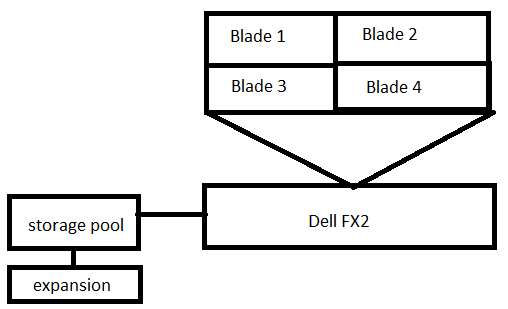
\includegraphics[scale = 0.70]{images/currentENV.png}
    \caption{TASI On-Premise Environment \textcolor{red}{(needs VISIO)} }
    \label{Current ENV}
\end{figure}

\begin{figure}[H]
\begin{center}
    \renewcommand{\arraystretch}{1.5}
    \begin{tabular}{|>{\raggedright\arraybackslash}l 
                    |>{\raggedright\arraybackslash}m{3cm}
                    |}
    \hline
    \rowcolor[HTML]{196fb4}\centering\textcolor{white}{\large Resource Type} 
                            & \centering\textcolor{white}{\large Resource Count (per Blade)} 
                            \tabularnewline 
    \hline
    CPU(s)              & 12 \\\hline
    Total cores         & XX \\\hline
    Memory              & 256GB RAM \\\hline
    Storage             & XX GB \\\hline
    Operating System    & ESXi 6.7 \\\hline
    \end{tabular}
\end{center}
\caption{Node count per Tenant}
\label{BLD-RSRC}
\end{figure}

\begin{figure}[H]
\begin{center}
    \renewcommand{\arraystretch}{1.5}
    \begin{tabular}{|>{\raggedright\arraybackslash}l 
                    |>{\raggedright\arraybackslash}l
                    |}
    \hline
    \rowcolor[HTML]{196fb4}\centering\textcolor{white}{\large Tenant} 
                            & \centering\textcolor{white}{\large Node Count} 
                            \tabularnewline 
    \hline
    Commonwealth of the Northern Mariana Islands (CNMI) & \vtop{\hbox{\strut (1) Primary CAS Controller }
                                                                \hbox{\strut (1) Backup CAS Controller}
                                                                \hbox{\strut (3) CAS Workers}}\\\hline
    All-Payer Claims Database (APCD)                    & \vtop{\hbox{\strut (1) Primary CAS Controller }
                                                                \hbox{\strut (1) Backup CAS Controller}
                                                                \hbox{\strut (3) CAS Workers}}\\\hline
    Centers for Medicare \& Medicaid Services (CMA)      & \vtop{\hbox{\strut (1) Primary CAS Controller }
                                                                \hbox{\strut (1) Backup CAS Controller}
                                                                \hbox{\strut (1) CAS Workers}}\\\hline
    Med-Quest                                           & \vtop{\hbox{\strut (1) Primary CAS Controller }
                                                                \hbox{\strut (1) Backup CAS Controller}
                                                                \hbox{\strut (1) CAS Workers}}\\\hline                                                            
    \end{tabular}
\end{center}
\caption{Resource count for a single Blade component.}
\label{TNTS-NDS}
\end{figure}

%----------------------------------------------------------------------------------%

\subsection{Design I}

The Design phase is a critical step in implementing a successful SAS infrastructure. During this phase, the technical specifications and architecture of the system are defined, and the appropriate hardware and software components are selected. This phase also includes creating a deployment plan, which outlines the steps for installing and configuring the system.

\subsubsection{Design Principles}

TASI will design a multi-tenant infrastructure that will accommodate all the VMs specified in the multi-tenancy configuration plan in Section \ref{Multi-Tenancy Configuration Plan}. The design should incorporate the architectural best practices of a \href{https://learn.microsoft.com/en-us/azure/well-architected/}{Well-Architected Framework}, which is a set design principles for running and designing workloads.

\begin{enumerate}
    \item Operational Excellence
    \begin{itemize}
        \item 
    \end{itemize}
    \item Reliability: A reliable application must be designed for failure by supporting high availability and disaster recovery principles. 
    \begin{itemize}
        \item CAS controller and CAS backup controller nodes must exist on separate hardware to support automated failover in the case of unexpected downtime. 
        \item TASI's on-premises infrastructure must have sufficient resources (e.g., compute, memory, storage) beyond the minimum requirement for supporting SAS technologies.
        \item All data that exists in volatile memory or storage should have regular backups. SAS loads data to be analyzed into non-volatile memory.
        \item All VMs should be scheduled for incremental backups and retention policies. 
    \end{itemize}
    \item Security: A secure application must be designed for confidentiality, integrity, and availability, whilst also adhering to new security standards such as authorization, encryption, monitoring, and auditing.
    \begin{itemize}
        \item Any data that TASI intends to store or process must comply with regulations and industry standards from HIPAA, UHM, RCUH, and other relevant compliance standards for protected health information.
        \item TASI must consider the principle of least privilege when designing an LDAP directory to support multi-tenancy.
        \item Data Governance: \textbf{\textcolor{red}{Fill me on May 24}}
        \item HIPPA compliance standards require data to be encrypted at-rest and in-transit. Data that is loaded in non-volatile memory for SAS, does not have to be encrypted. 
        \end{itemize}
    \item Performance Efficiency: An efficient application has the ability to use computing resources efficiently to meet system requirements, and maintains that efficiency as demand and technology changes.
    \begin{itemize}
        \item CAS worker nodes must be configured for MPP mode, where possible. 
        \item The SAS environment must be designed on infrastructure with ample resources beyond the minimum requirements to prevent potential bottlenecks as demand scales up.
        \item TASI must ensure that the servers have sufficient resources beyond the minimum requirements for VMs, to prevent potential bottlenecks when demand increases. 
        \item As the infrastructure grows, TASI must consider load balancing applications for user traffic across multiple servers. 
        \item To prepare for MLA II (VM Migration), TASI must ensure that their initial deployment is loosley coupled for scalability. This involves designing the infrastructure to be elastic, so it can handle sudden spikes in demand without compromising performance or availability.
    \end{itemize}
    \item Cost Optimization
    \begin{itemize}
        \item We will not have true cost optimization as we are using the CAPEX model. 
    \end{itemize}
\end{enumerate}

\subsubsection{IAM Design}

RCUH and UHTASI.

if uh then uh makes their own active directory. (check asana cause athena is working on that information with its

if tasi, we have to design our own LDAP system which is goin gto suck 

[user] -> [vpn] -> [connection is approved by LDAP]

\subsubsection{Multi-Tenancy}

The initial deployment of MLA will involve the installation of SAS 9.4 and SAS Viya 3.5 on existing infrastructure. The deployment configuration for each tenant will be tailored to meet their individual requirements. 

\begin{figure}[H]
    \centering
    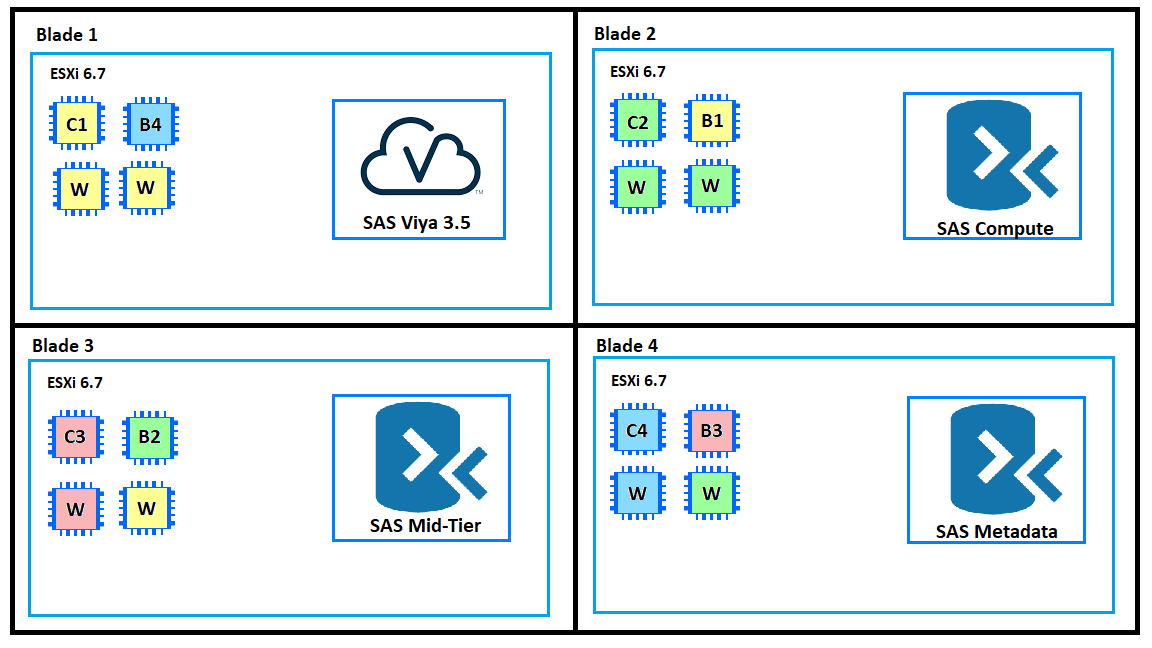
\includegraphics[scale = 0.52]{images/initial-deployment-diagram.png}
    \caption{Multi-Tenant Deployment \textcolor{red}{(needs VISIO)} }
    \label{Initial Multi-Tenant Deployment}
\end{figure} 

To maximize resource efficiency, CAS nodes will be evenly distributed across each blade, where a blade will consist of one controller, one backup controller, and two workers. The controller and backup controller, configured on the same system, will belong to separate tenants. The workers will also belong to separate tenants but each blade will have at least one related controller and worker per system. 

Subsequently, four additional VMs will be created to support the installation of SAS Viya 3.5 and SAS DMA. SAS Viya 3.5 will be installed as software on top of a RHEL 3.7X VM instance, in Blade 1. SAS DMA consists of three software components that will installed as software on top of Windows Server 2019 VM instances, in Blades' 2, 3, and 4. 

%----------------------------------------------------------------------------------%
\subsection{Implementation I}

April 18, 2023:
SAS 9.4 is installed first on TASI system. It is configured this way on blade 1. 

%----------------------------------------------------------------------------------%

\subsection{Testing \& Integration I}

%----------------------------------------------------------------------------------%

\subsection{Operations \& Maintenance I}
\newpage

%Creates the HCI section. 
\section{Hyper-Converged Infrastructure (HCI)} \label{section: HCI}

HCI, or Hyper-Converged Infrastructure, is a software-defined, unified system that combines the traditional elements of IT infrastructure (e.g., compute, networking, management, storage) with virtualization, simplifying infrastructure, reducing costs, and increasing scalability and flexibility. In a traditional IT Infrastructure, servers, storage networks, and storage systems are physically separated as stand alone hardware devices (e.g., servers, network switches, disk arrays). Consolidating these components into a single, integrated system simplifies the management, deployment, configuration, and maintenance of your IT Infrastructure. 

The benefits of an HCI environment include: 
\begin{itemize}
    \item Scalability: Designed to scale out by adding additional nodes on-demand to your system.
    \item Efficiency: Improve resource utilization by using or eliminating idle storage capacity.
    \item Agility: Quickly deploy new applications and workloads without extensive planning across systems. 
    \item Data Protection: Integrated backup and disaster recovery.
    \item Reduced Hardware Costs: Reduce the amount of hardware required reducing CAPEX\footnote{Capital expenditure is the cost a business incurs to acquire assets that will provide benefits beyond the current year.}/OPEX\footnote{Operating expenses refer to the money a company spends to run day-to-day operations.} costs. 
\end{itemize}

% Single-Machine HCI Relationship with Cloud Deployments %
%\begin{figure}[H]
%    \centering
%    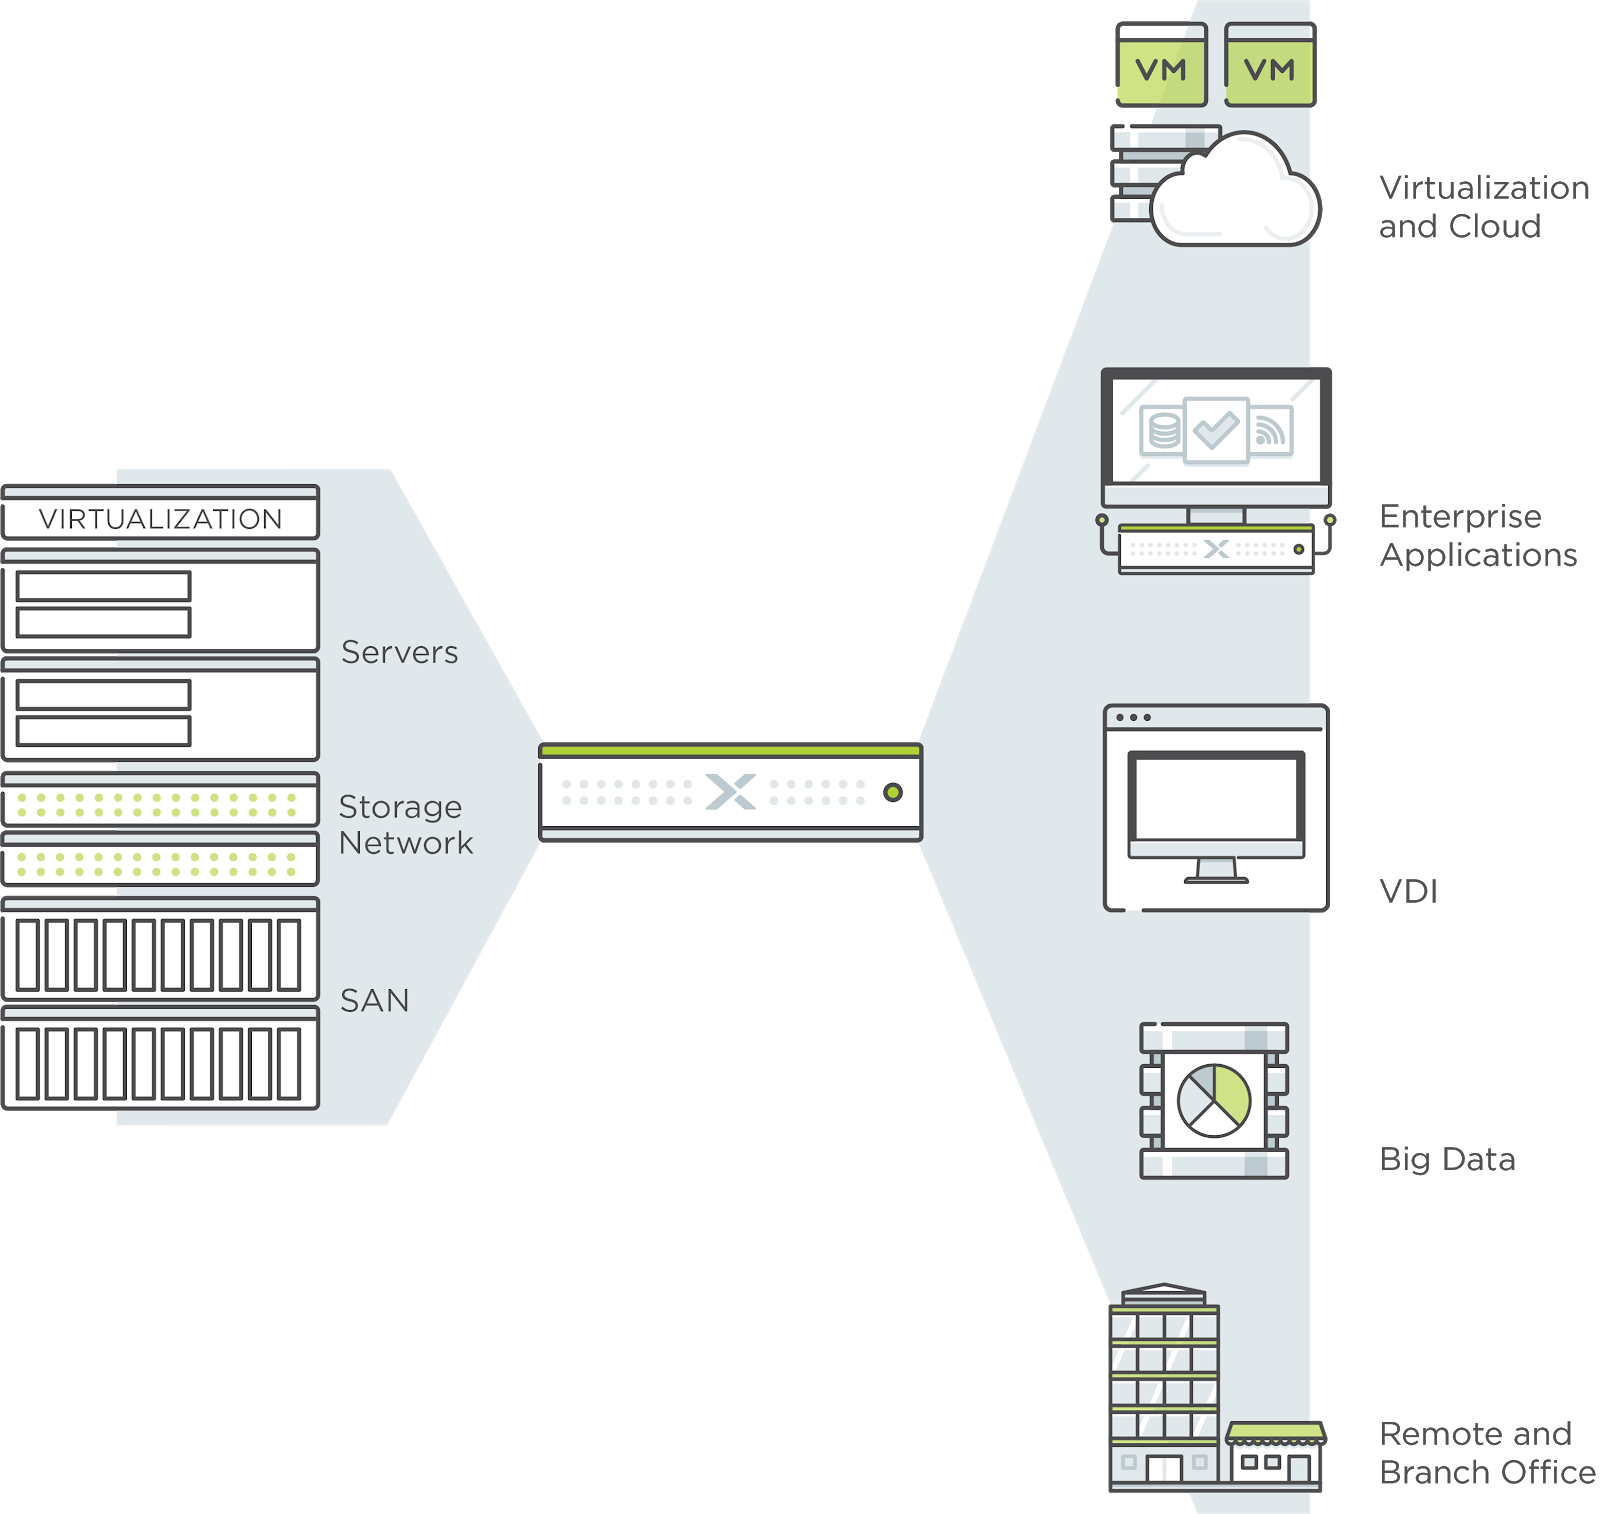
\includegraphics[scale = 0.25]{images/HCI_Nutanix_Node.png}
%    \caption{Single-Machine HCI \textcolor{red}{(STOLEN EXAMPLE)}}
%    \label{HCI Explained (Single-Machine)}
%\end{figure}

\begin{figure}[H]
    \centering
    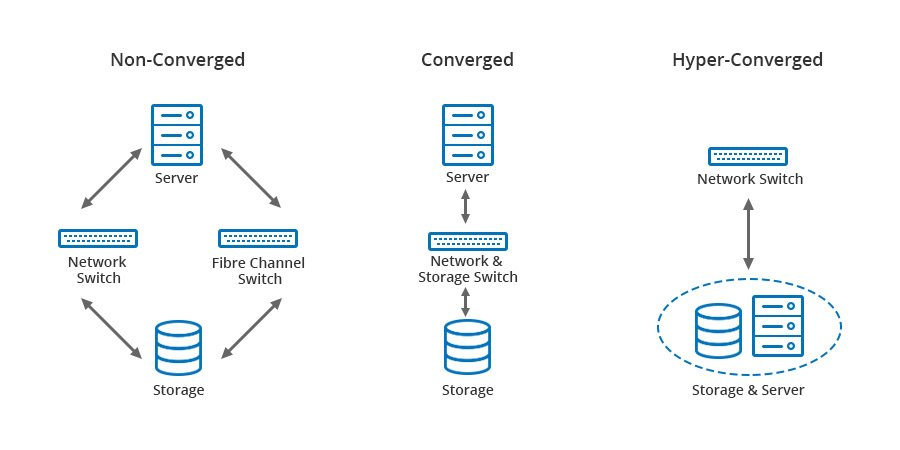
\includegraphics[scale = 0.5]{images/HCI_tldr.jpg}
    \caption{Types of IT Infrastructures \textcolor{red}{(STOLEN EXAMPLE)}}
    \label{HCI Convergance Comparison}
\end{figure}

In HCI, multiple servers or nodes are combined to create a cluster. These nodes share their computing and storage resources with each other to create a multi-purpose integrated system. The design of your HCI cluster will depend on your specific needs and requirements.

The software that powers HCI also includes a management layer, which automates tasks like resource provisioning, data migration, and load balancing. This layer abstracts the hardware, making it easier to manage and deploy your IT infrastructure. Overall, HCI is a powerful and flexible solution that can help organizations streamline their IT operations, reduce costs, and improve efficiency.


\newpage

%Creates the Massively Learning Activities section.
\section{Massively Learning Activities II - Migration Deployment} \label{section: MLA2}
TASI has been contracted by CNMI to create an infrastructure that allows for data analytics on Protected Health Information (PHI). This infrastructure will initially be hosted on-premises, with plans to move towards a hybrid solution in the future. To achieve this, we will be providing a Platform as a Service (PaaS) solution, by hosting SAS Viya services on our own hardware and allowing tenants to access and utilize the platform for their own analytics applications.

The tenants, including APCD, CMNI, CMA, Criminal Justice, and several Education environments, will provide the necessary data, which will be submitted to an ETL data pipeline for processing before being sent to SAS on-prem servers. Once the data has been processed, tenants may perform data analytics using advanced algorithms in SAS programming language.

To ensure secure operations, we will configure the security relationships between the software, hardware, and tenants using LDAP, security groups, encryption  and other related tools. Our goal is to architect a high-performance infrastructure that allows for advanced data analytics while maintaining the confidentiality and security of PHI.

Due to SAS being a time sensitive project, the initial deployment will have SAS suites and VMs installed on existing hardware, with plans to migrate the infrastructure to newly acquired hardware in the future.

The final and completed deployment of SAS Viya 3.5 will expect a total of 8 tenants:

\begin{enumerate}
    \item Commonwealth of the Northern Mariana Islands (CNMI)
    \item All-Payer Claims Database (APCD)
    \item Centers for Medicare \& Medicaid Services (CMA)
    \item Med-Quest
    \item University Education 1
    \item University Education 2
    \item University Education 3
    \item University Education 4
\end{enumerate}

\subsection{Planning II}

The System Development Lifecycle (SDLC) is a project management model that defines different stages that are necessary to bring a project from conception to deployment and later maintenance. The SDLC model consists of several phases, which typically include requirements gathering, design, development, testing, deployment, and maintenance. The specific activities within each phase may vary depending on the project and the organization, but the basic principles are the same. The SDLC model is a flexible framework that can be adapted to suit the needs of different projects and organizations. It provides a systematic approach to software development that helps ensure that software is built efficiently, effectively, and with minimal risk.

Massively Learning Activities will follow a similar variation to the SDLC project management model where each SDLC stage will correspond to a subsection in this chapter. 

\subsection{Required of Analysis II}
\begin{itemize}
    \item Requirement of Analysis
    \item Deployment Design
\end{itemize}

\subsection{Design II}
We will be using VMotion to migrate virtual machines. 

\subsection{Implementation II}

\subsection{Testing \& Integration II}

\subsection{Operations \& Maintenance II}


\newpage

% Copy this to add more chapters
%\section{Copy me} \label{section: copy me}
\lipsum[1-8]
%\newpage

% Creates references using the Biblatex 
%\bibliographystyle{plain}
%\bibliography{General/References.bib}
%\newpage

\appendix % Any section after this command will have a letter as an index

% Adds an appendix entry
\section{Appendix A title} \label{section: appendix A title}
\lipsum[1-8]
\newpage

\end{document}
